\section{Numerical Results and Discussion}
\label{sec:results}

\subsection{Optimized Designs}
As mentioned earlier, the mass sensitivity study focused on two
objective functions, substructure mass and capital cost.  It is worth
reiterating here that the design variables are only focused on the
substructure.  From the freeboard (\unit[10]{m} above the waterline in
this application) and up, including the tower, nacelle, and rotor, the
design was frozen to the DTU \unit[10]{MW} Reference Turbine
\citep{dtu10mw}.  From the freeboard and down, the design was subject to
optimization.  Furthermore, while this paper has espoused a system
approach for an offshore wind energy system, including lifecycle costs
and operations, this study is focused purely on traditional substructure
engineering as a first foray into the tool's capability.

\subsubsection{Caveats}
It should be noted that the arrival at \textit{optimized} designs here,
means strictly optimized in the convergence of the optimization
algorithm around the WISDEM model of a floating offshore turbine.  It is
not an optimized design in that it would outperform other designs or be
considered ready for manufacturing.  It is merely optimized for the set
of assumptions, load cases, and physics models used by WISDEM.  Given
the description of \textit{FloatingSE} in this paper, these assumptions
and modeling limitations are numerous and include,
\begin{itemize}
\item Hydrostatic loading only, no hydrodynamic loads, effects, or
  considerations (except for eigenmodes).  Therefore, design features
  meant to handle or minimize dynamic loading are not present;
\item Single load case only, the maximum thrust condition.  Design
  features for other DLCs, such as mooring line snap, are not present;
\item Static load analysis only (except for eigenmodes);
\item Simple beam-based finite element structural analysis.  Because of
  this, and other assumptions in the structural analysis, connecting
  pontoons appear much larger than they would otherwise have to be;
\item Quasi-static mooring analysis;
\item Simplified capital cost modeling, frequently based on mass
  scaling.  Costs of highly tapered columns, joints, complicated welding
  connections are not included, so these features are sometimes included
  by the optimizer;
\item Modeling of substructure capital costs only, no manufacturing,
  assembly, installation, operations, or maintenance costs captured.
  This means that the TLP looks like the lowest cost option for now,
  but that answer could change when other costs are considered;
\item Incomplete incorporation of existing codes, standards, and best
  practices.
\end{itemize}

\subsubsection{Depiction}
Results of the design optimization are shown both visually and in
tabular form in Table \ref{tbl:optdesign}.  The optimized substructure
designs are shown in Figures
\ref{fig:spar-design}--\ref{fig:tlp-design}.  To understand the
visualizations, the sea floor is shown in the light brown beneath the
substructure and the ragged aqua plane is the waterline.  The
alternating dark/light gray colors of the substructure show the
different sections in the geometry discretization.  The darker brown
coloration at the bottom of the columns is the permanent ballast and the
blue color shows the water ballast.  Mooring lines are shown in green.
Pontoons, whether connecting the columns or the mooring lines, are shown
in red.

\begin{table}[htbp]
  \begin{center}
    \caption{Nacelle and RNA mass perturbations for design sensitivity studies.}
    \label{tbl:optdesign}
    {\small
    \begin{tabular}{l|cc|cc|cc}
      \hline
       & \multicolumn{2}{c|}{\textbf{Spar}} & \multicolumn{2}{c|}{\textbf{Semi}} & \multicolumn{2}{c}{\textbf{TLP}}\\
      Objective function & Mass & Cost & Mass & Cost & Mass & Cost\\ \hline \hline
Substructure mass [1000t] & 10.2 & 15.0 & 16.1 & 16.8 & 4.2 & 6.2\\
Substructure cost [M USD] & 21692.8 & 18028.0 & 18038.1 & 18100.4 & 3342.5 & 2687.5\\
Substructure displacement [k$m^3$] & 18.6 & 17.2 & 21.5 & 21.6 & 8.2 & 7.9\\
Substructure main col mass [1000t] & 6.8 & 10.5 & 8.8 & 9.4 & 0.7 & 0.8\\
Substructure offset col mass [1000t] &  &  & 1.0 & 1.0 &  & \\
Substructure main ballast mass [t] & 2340.9 & 6895.6 & 8137.7 & 8790.3 & 20.8 & 282.2\\
Substructure offset ballast mass [t] &  &  & 227.1 & 226.3 &  & \\
Substructure water ballast [1000t] & 6.0 & 0.8 & 1.7 & 1.2 & 1.5 & 0.1\\
Main column draft [m] & 131.4 & 91.0 & 13.5 & 13.8 & 15.4 & 9.8\\
Offset column draft [m] &  &  & 14.0 & 13.9 &  & \\
Mooring downward force [MN] & 27.4 & 18.2 & 41.0 & 40.4 & 27.0 & 17.6\\
Main column ave diameter [m] & 12.4 & 13.0 & 11.9 & 11.9 & 10.3 & 8.2\\
Offset column ave diameter [m] &  &  & 10.1 & 10.1 &  & \\
Main column ave thickness [mm] & 65.4 & 71.9 & 50.4 & 50.5 & 45.8 & 53.3\\
Offset column ave thickness [mm] &  &  & 53.3 & 53.2 &  & \\
\hline
Substructure main col costs [M USD] & 21670.8 & 17997.1 & 6297.6 & 6346.7 & 3338.4 & 2671.7\\
Substructure offset col costs [M USD] &  &  & 3894.3 & 3898.9 &  & \\
Substructure main ballast cost [M USD] & 234.1 & 689.6 & 813.8 & 879.0 & 2.1 & 28.2\\
Substructure offset ballast cost [M USD] &  &  & 22.7 & 22.6 &  & \\
Mooring cost [M USD] & 21.9 & 24.1 & 52.1 & 51.7 & 4.0 & 3.4\\
      \hline
    \end{tabular}
    }
  \end{center}
\end{table}


\subsubsection{Optimized Spar Design}

\begin{figure}[htb]
  \begin{subfigure}[b]{0.24\linewidth}
    \centering 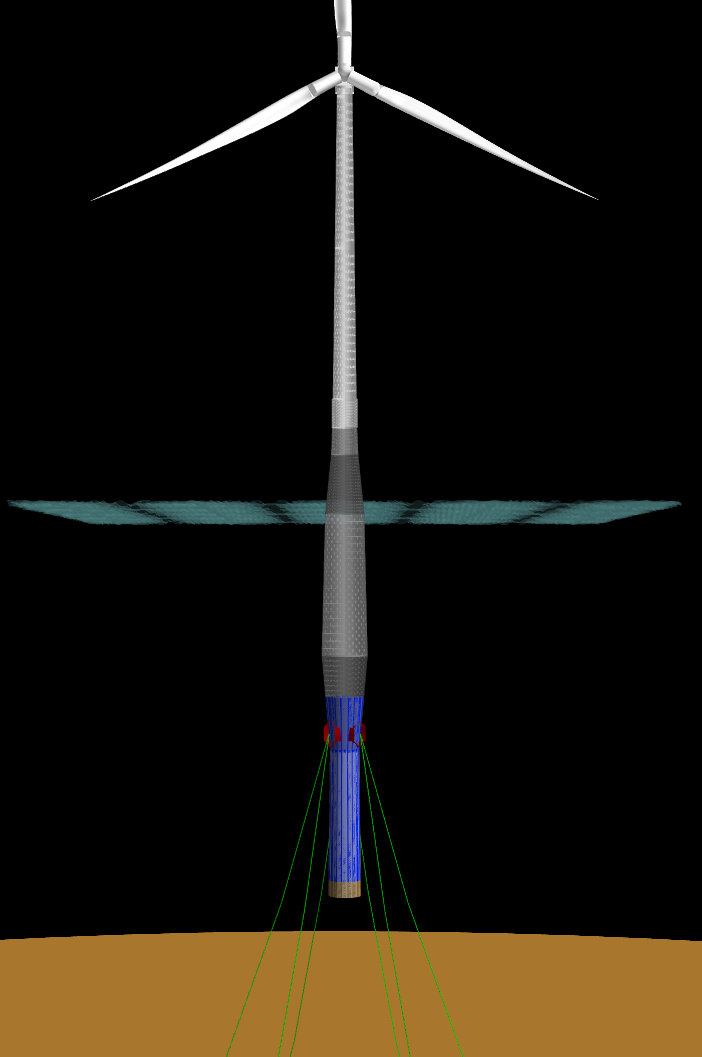
\includegraphics[height=2.25in]{spar-mass1.png}
    \caption{Mass-optimized}
  \end{subfigure}
  \begin{subfigure}[b]{0.24\linewidth}
    \centering 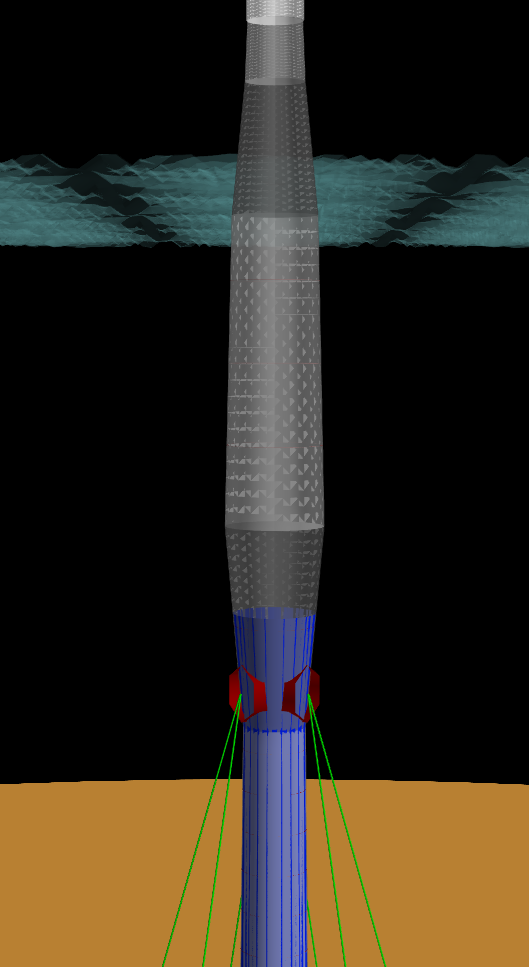
\includegraphics[height=2.25in]{spar-mass2.png}
    \caption{Mass-optimized}
  \end{subfigure}
  \begin{subfigure}[b]{0.24\linewidth}
    \centering 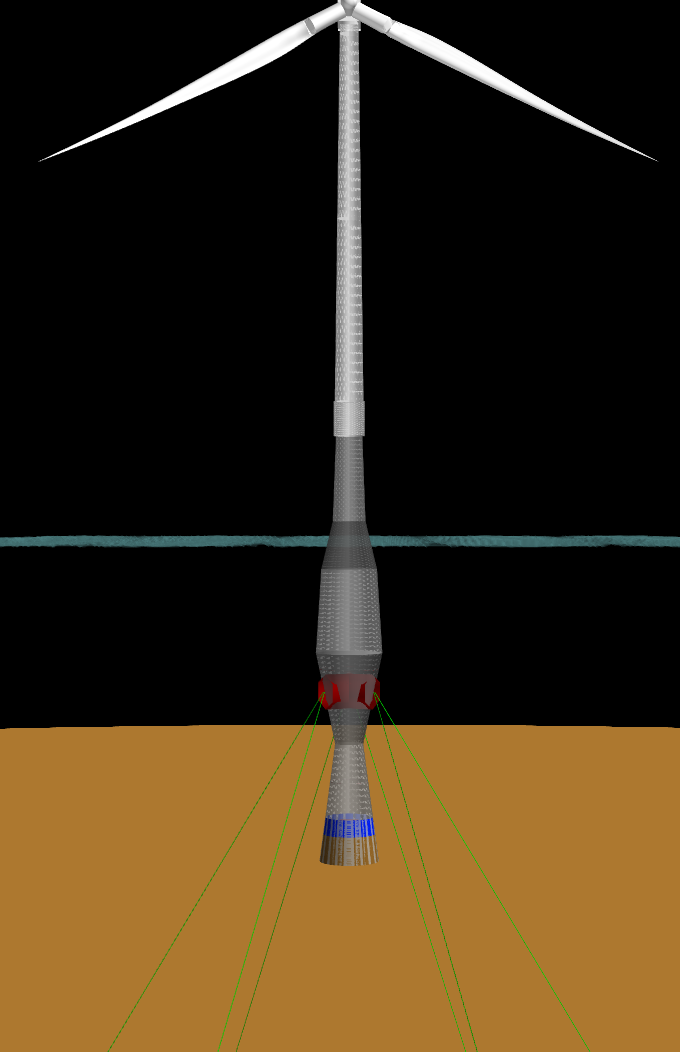
\includegraphics[height=2.25in]{spar-cost1.png}
    \caption{Cost-optimized}
  \end{subfigure}
  \begin{subfigure}[b]{0.24\linewidth}
    \centering 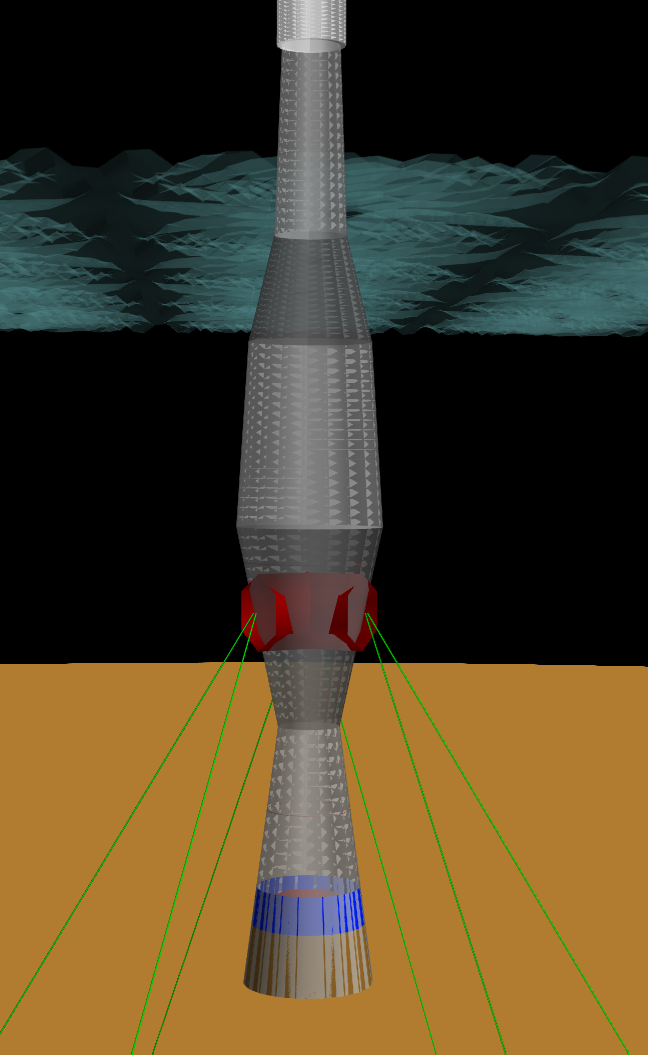
\includegraphics[height=2.25in]{spar-cost2.png}
    \caption{Cost-optimized}
  \end{subfigure}
  \caption{Views of optimized spar substructure designs.}
  \label{fig:spar-design}
\end{figure}

The optimized spar designs are shown in Figure \ref{fig:spar-design},
with obvious differences between the mass-optimized and cost-optimized
designs.  The mass-optimized design has a deeper draft with a narrower
diameter and significantly more water ballast.  The cost-optimized
design has a wider diameter with a shorter draft, more permanent
ballast, and less water ballast.  The differences are driven by the fact
that water ballast is not counted as part of the manufactured mass, so
when minimizing mass, the optimizer has traded permanent for water
ballast.  To ensure stability, since water ballast is less dense than
permanent ballast, a deeper draft was needed.  In contrast, when
optimizing for cost, a shorter draft means less rolled steel
columns, which are expensive, and thus the heavier, permanent ballast is
required for stability.

Both designs have a number of similarities as well.  The column diameter
narrows slightly near the mooring attachment points.  Also, there are
three mooring attachment points, with two catenary lines per connection
for a total of six lines and anchors.

\subsubsection{Optimized Semisubmersible Design}

\begin{figure}[htb]
  \begin{subfigure}[b]{0.29\linewidth}
    \centering 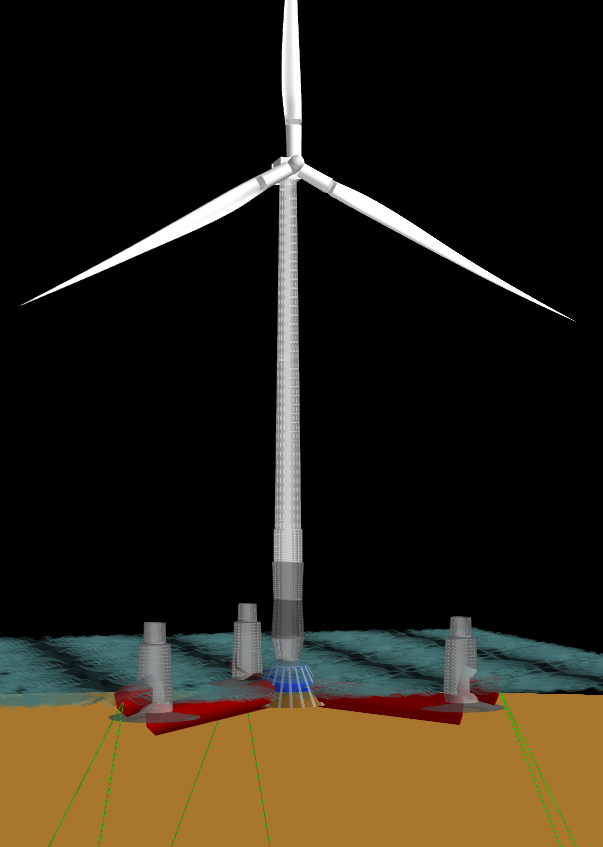
\includegraphics[height=2.25in]{semi-mass1.png}
    \caption{WISDEM semisubmersible}
  \end{subfigure}
  \begin{subfigure}[b]{0.40\linewidth}
    \centering 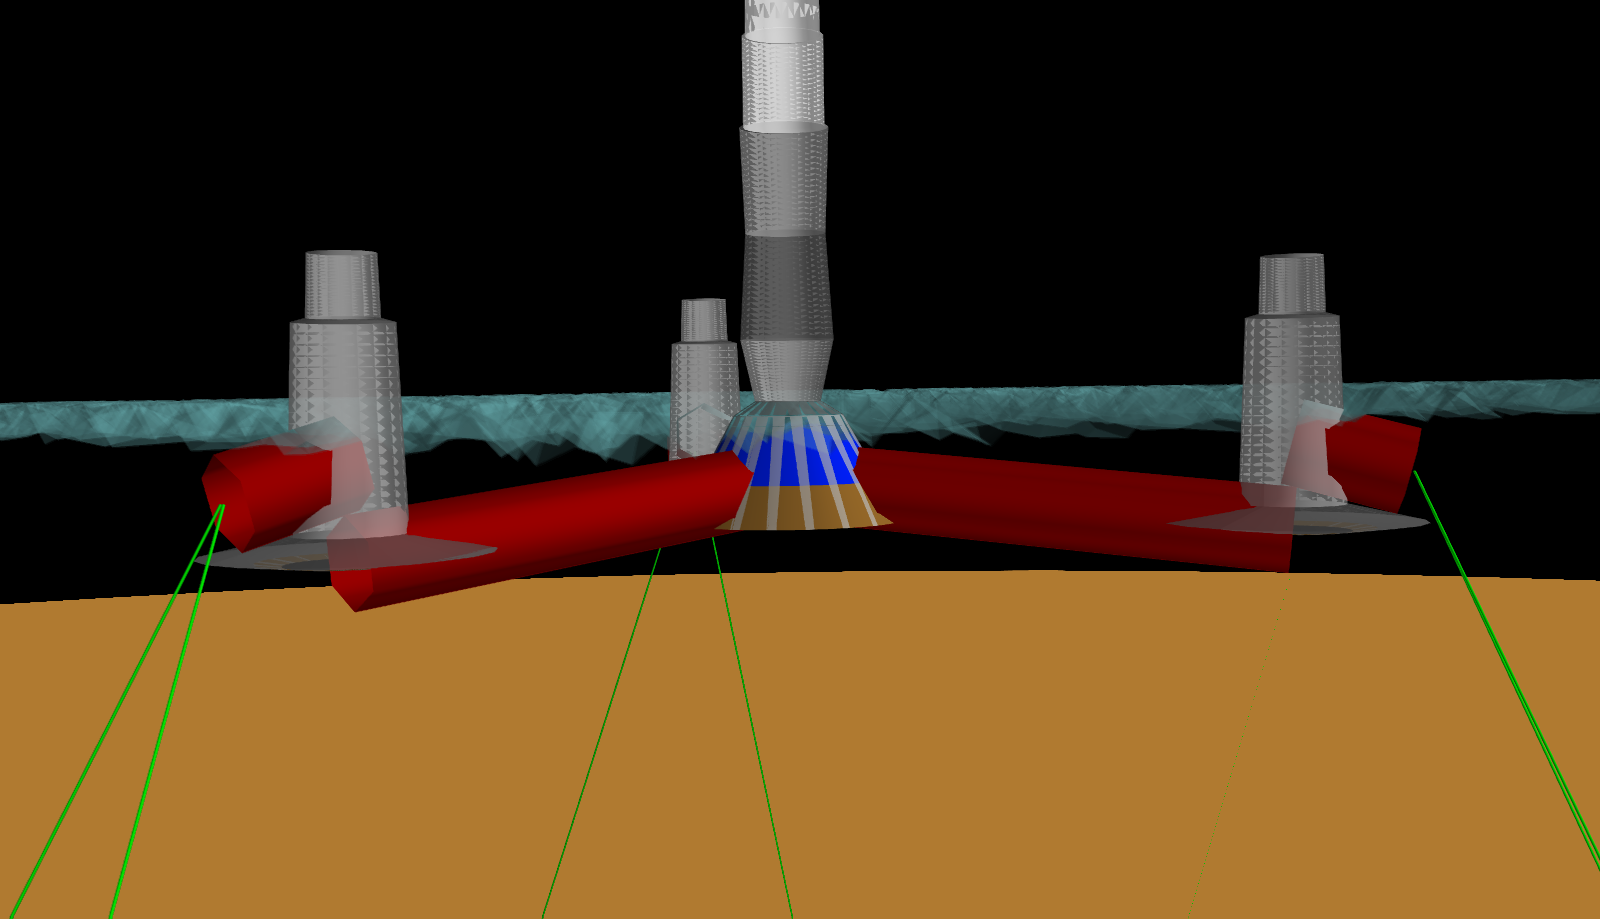
\includegraphics[width=0.95\textwidth]{semi-mass2.png}
    \caption{WISDEM semisubmersible}
  \end{subfigure}
  \begin{subfigure}[b]{0.29\linewidth}
    \centering 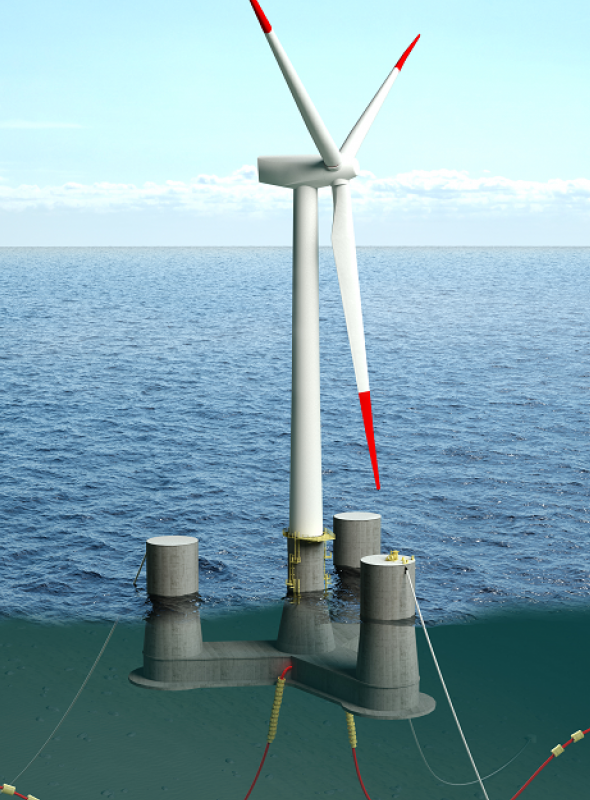
\includegraphics[height=2.25in]{oo-star.png}
    \caption{OO-Star Wind Floater}
  \end{subfigure}
  \caption{Views of semisubmersible substructure optimized for minimal
    substructure mass (not including the mooring system) in (a) and (b).
    OO-Star Wind Floater design by Dr.techn.Olav Olsen for the LIFES50+
    project, a European Horizon 2020 funded program, in (c).}
  \label{fig:semi-mass}
\end{figure}

The optimized semisubmersible design is shown in Figure
\ref{fig:semi-mass}a--b.  In this case, the mass- and cost-optimized
designs look nearly identical, so only one is shown (mass-optimized).
There are three offset columns that sit \unit[53.8]{m} away from the
central column and are connected with a single pontoon.  Near
the bottom, the diameter flares to add some permanent ballast without a
significant increase in column length.  Two catenary mooring lines
attach to each offset column.  The main column has a bell-bottom shape
at the keel with approximately equal volumes of permanent and water
ballast.

It is interesting to compare the semisubmersible design created by
WISDEM to other semisubmersible designs created for the DTU
\unit[10]{MW} reference turbine.  The LIFES50+ project generated a few
candidate substructure designs using the same reference turbine, two of
which were semi-submersibles.  One of those designs, the OO-Star Wind
Floater created by Dr.techn.Olav Olsen, a Norwegian marine consulting
company, has a similar configuration and is shown in Figure
\ref{fig:semi-mass}c. The similarities are especially interesting given the
low-fidelity resolution of the physics and the many simplifying
assumptions used in \textit{FloatingSE}. Unfortunately, despite the
configuration similarities, the OO-Star Wind Floater is made out of
concrete, instead of steel, so direct comparison of dimensions and
weights is not practical.

\subsubsection{Optimized Tension Leg Platform Design}

\begin{figure}[htb]
  \begin{subfigure}[b]{0.24\linewidth}
    \centering 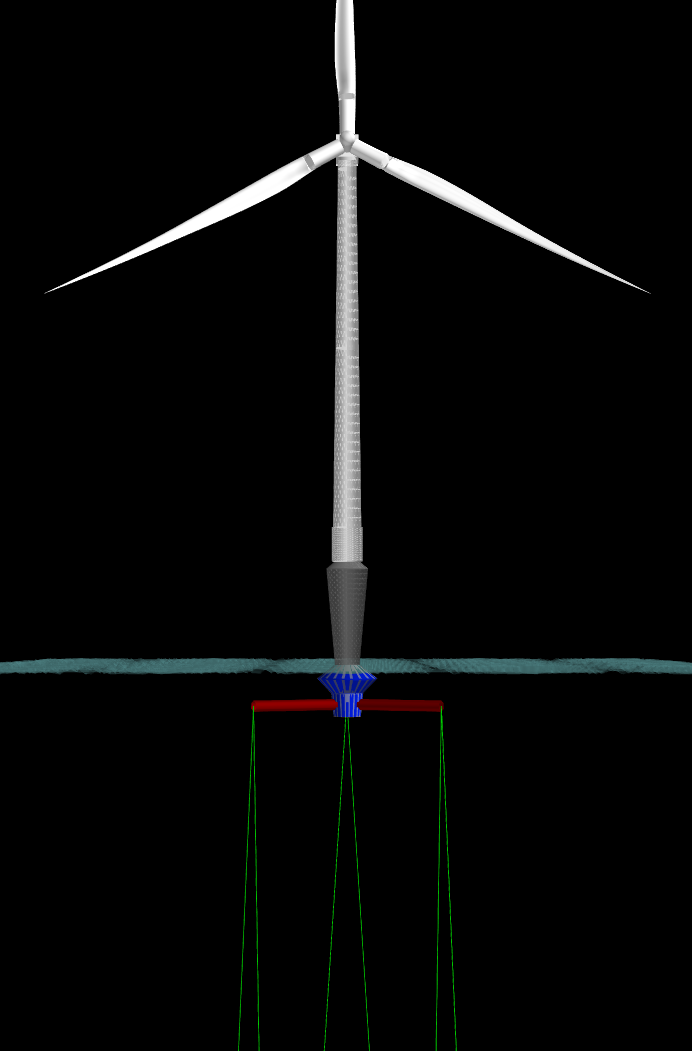
\includegraphics[height=2in]{tlp-mass1.png}
    \caption{Mass-optimized}
  \end{subfigure}
  \begin{subfigure}[b]{0.24\linewidth}
    \centering 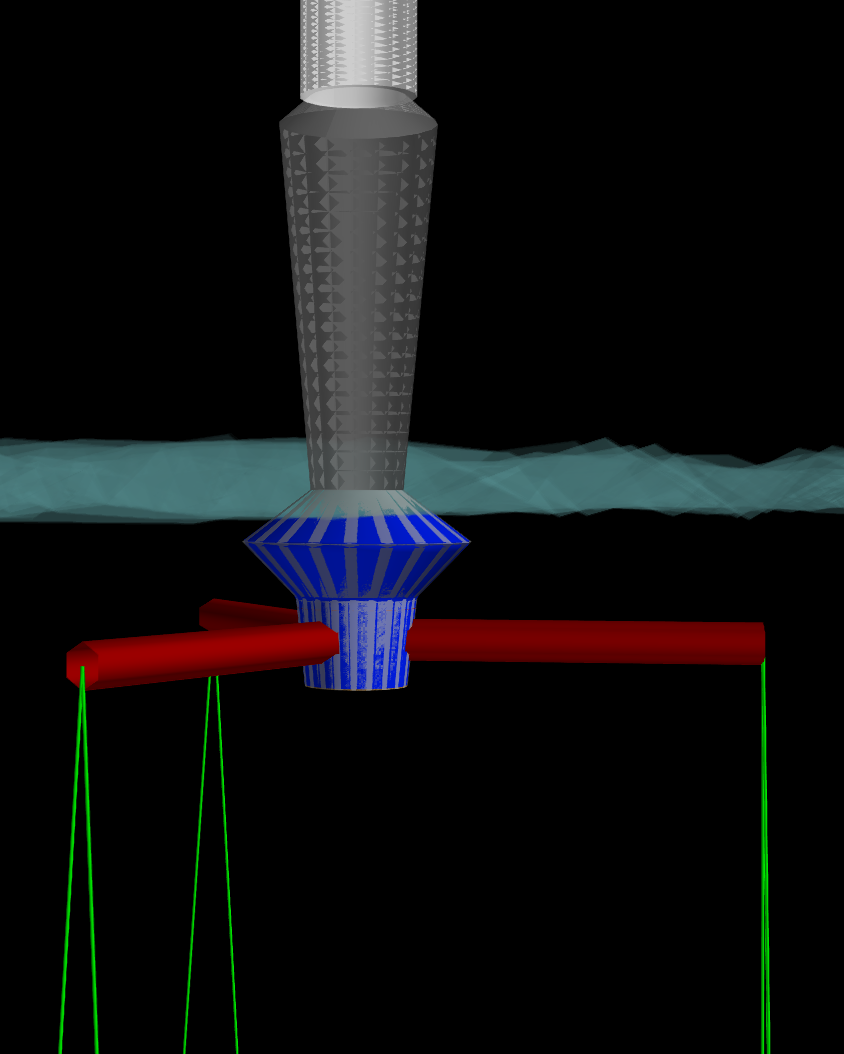
\includegraphics[height=2in]{tlp-mass2.png}
    \caption{Mass-optimized}
  \end{subfigure}
  \begin{subfigure}[b]{0.24\linewidth}
    \centering 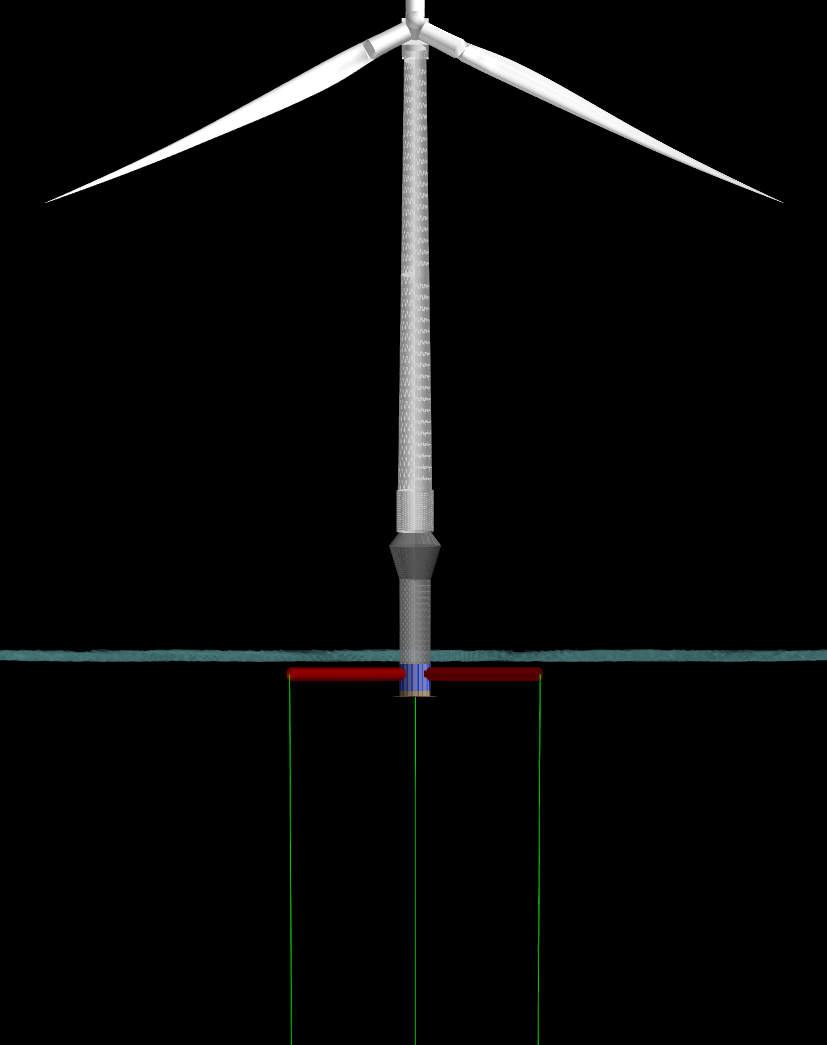
\includegraphics[height=2in]{tlp-cost1.png}
    \caption{Cost-optimized}
  \end{subfigure}
  \begin{subfigure}[b]{0.24\linewidth}
    \centering 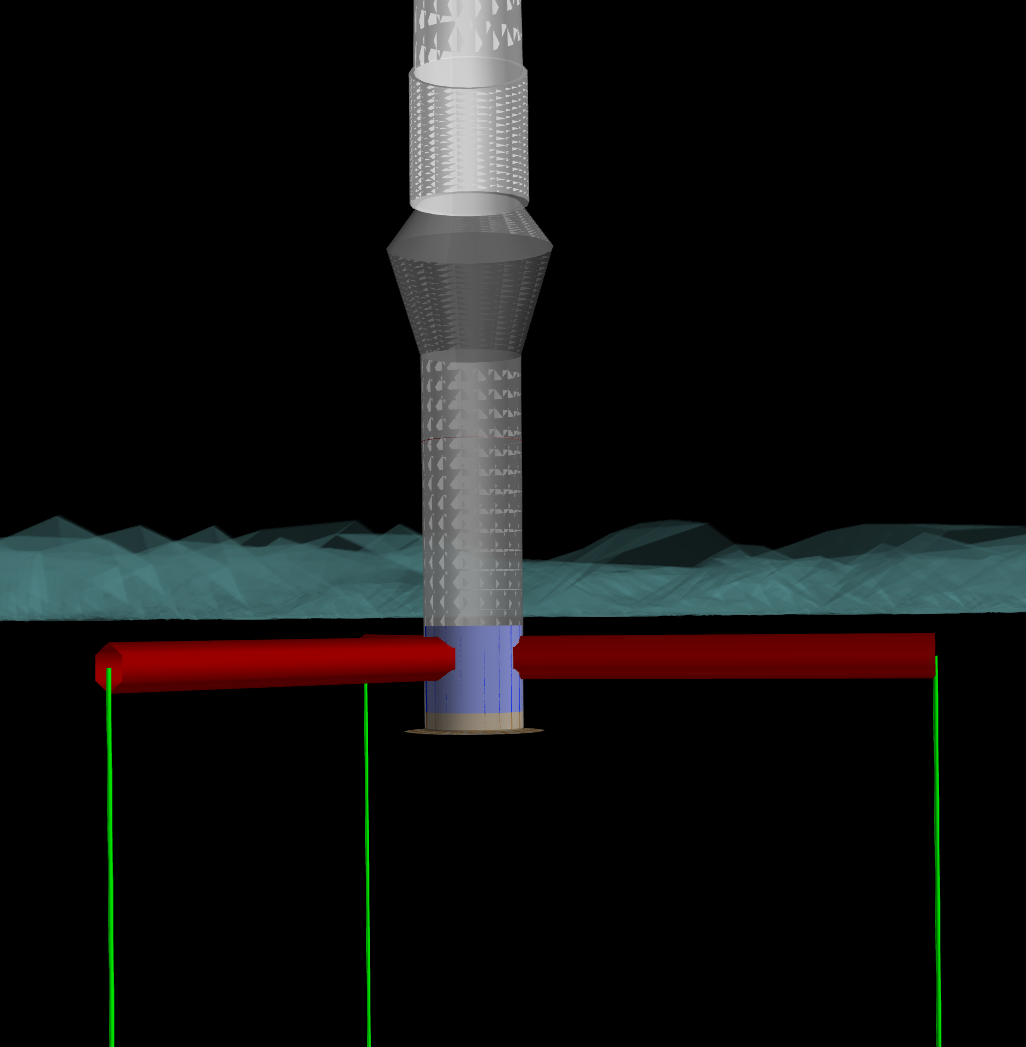
\includegraphics[height=2in]{tlp-cost2.png}
    \caption{Cost-optimized}
  \end{subfigure}
  \caption{Views of optimized TLP substructure designs.}
  \label{fig:tlp-design}
\end{figure}

The TLP designs are shown in Figure \ref{fig:tlp-design}, and
differences between the mass- and cost-optimized geometries are once
again obvious.  The mass-optimized design has three legs with two taut
mooring lines per attachment and, as with the spar design, extensive use
of water ballast.  The legs extend \unit[30.5]{m} from the centerline to
the mooring attachment points.  In contrast, the cost-optimized design
has a single taut mooring line per attachment and requires very little
ballast.  This difference is driven primarily by the decision to not
include the mooring system into the substructure mass budget.  Table
\ref{tbl:optdesign} shows that the total mooring downward force on the
structures.  Despite needing sturdier legs to support those mooring
loads, shifting additional stability burden to the mooring system allows
for a lighter structure.

\subsection{Sensitivity Studies}

\begin{table}[htbp]
  \begin{center}
    {\small
    \caption{Nacelle and RNA mass perturbations for design sensitivity studies.}
    \label{tbl:delta_rna}
    \begin{tabular}{cccc}
      \hline
      \textbf{Nacelle Perturbation} & \textbf{Nacelle Mass [\unit{kg}]} & \textbf{RNA Mass [\unit{kg}]} &
      \textbf{RNA Perturbation}\\ \hline \hline
      Nominal & 446,036 & 672,301 & -\\
      +10\% & 490,640 & 716,904 & +6.6\%\\
      -10\% & 401,433 & 627,697 & -6.6\%\\
      -25\% & 334,527 & 560,791 & -16.6\%\\
      -33\% & 297,506 & 523,770 & -22\%\\
      -50\% & 223,018 & 449,282 & -33\%\\ \hline
    \end{tabular}
    }
  \end{center}
\end{table}

For the sensitivity studies, the optimized designs shown above were
taken as baseline starting points.  Then, the DTU 10MW reference turbine
nacelle mass was perturbed away from its nominal value by the
parameterization shown in Table \ref{tbl:delta_rna}.  Next, each design
was re-optimized at the new nacelle mass value using the Nelder-Mead
Simplex algorithm.  All continuous design variables, constraints, and
their bounds were kept consistent from the baseline optimization.  The
integer design variables were dropped to focus on a neighborhood search.
As above, two sets of sensitivity optimizations were performed with
different objective functions: one for substructure mass (not including
the mooring system), and one for total substructure mass (including the
mooring system).

\subsubsection{Caveats}
All of the caveats regarding substructure design mentioned above still
apply to the design sensitivity analysis as well.  In addition to those,
there are a couple of other points to keep in mind when considering the
results shown here,
\begin{itemize}
\item Design variables did not include the tower, a key structural
  component that would change with nacelle mass.  Had tower design
  variables been included, the total mass reductions would likely have
  been higher;
\item Cost sensitivity is for substructure capital cost only.  Other
  costs such as those captured in a balance of station or operational
  model would likely demonstrate different sensitivities;
\item The cost rates listed in Table \ref{tbl:factors} are notional,
  but still determine the priorities of the cost-optimized solutions and
  break-even cost points.  Thus, the final break-even costs should also
  be considered notional;
\item Just as the optimized designs reflect the assumptions and
  fidelity of \textit{FloatingSE}, so too do the sensitivity study
  results.  So, if the underlying assumptions or fidelity improve in
  the future, the key points determined here may shift.
\end{itemize}


\subsubsection{Mass-Optimized Design Sensitivity}
The sensitivity of substructure mass (not including the mooring system),
for all three substructure types, with respect to changes in nacelle
mass is shown in Figure \ref{fig:mass-mass}.  Absolute values of mass
changes are shown in Figure \ref{fig:mass-mass}a and percentage changes
are in Figure \ref{fig:mass-mass}b.  Reading from right to left, between
the three substructure types, the slopes are all initially similar, but
not exactly the same.  The slope of the spar curve appears the most
linear and the steepest, with approximately \unit[1.5--2]{kg} of
substructure mass removed for each \unit[1]{kg} of mass removed from the
nacelle.  The slope for the TLP is shallower, approximately
\unit[1]{kg} of substructure mass removed for each \unit[1]{kg} of
mass removed from the nacelle.  The slope of the semisubmersible curve is
the most interesting.  For small deviations around the nominal point,
the slope of the semisubmersible curve nearly matches that of the spar,
but at more significant mass decreases, the slope flattens out and the
substructure mass is relatively constant.  This implies that the
substructure design is more heavily bracketed by constraints and design
variable bounds.

\begin{figure}[htb]
  \begin{subfigure}[b]{0.49\linewidth}
    \centering 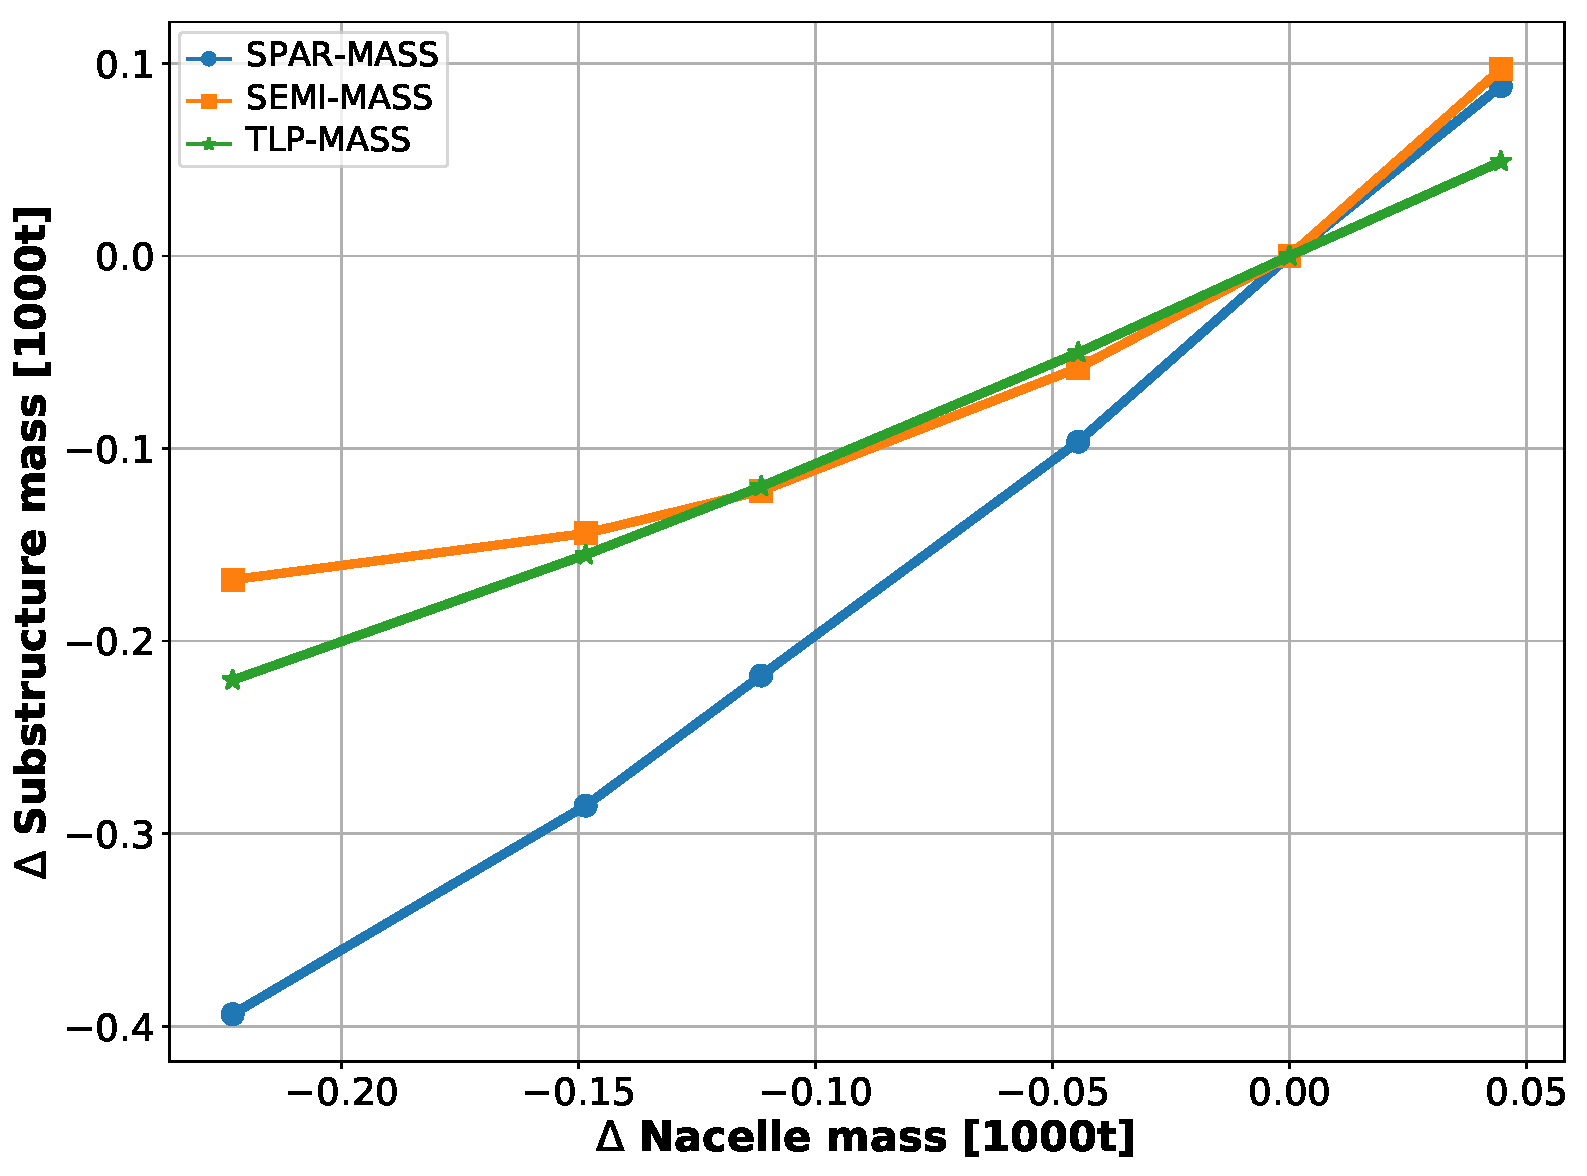
\includegraphics[width=0.9\textwidth]{mass-mass}
    \caption{Absolute mass changes, mass-optimized}
  \end{subfigure}
  \begin{subfigure}[b]{0.49\linewidth}
    \centering 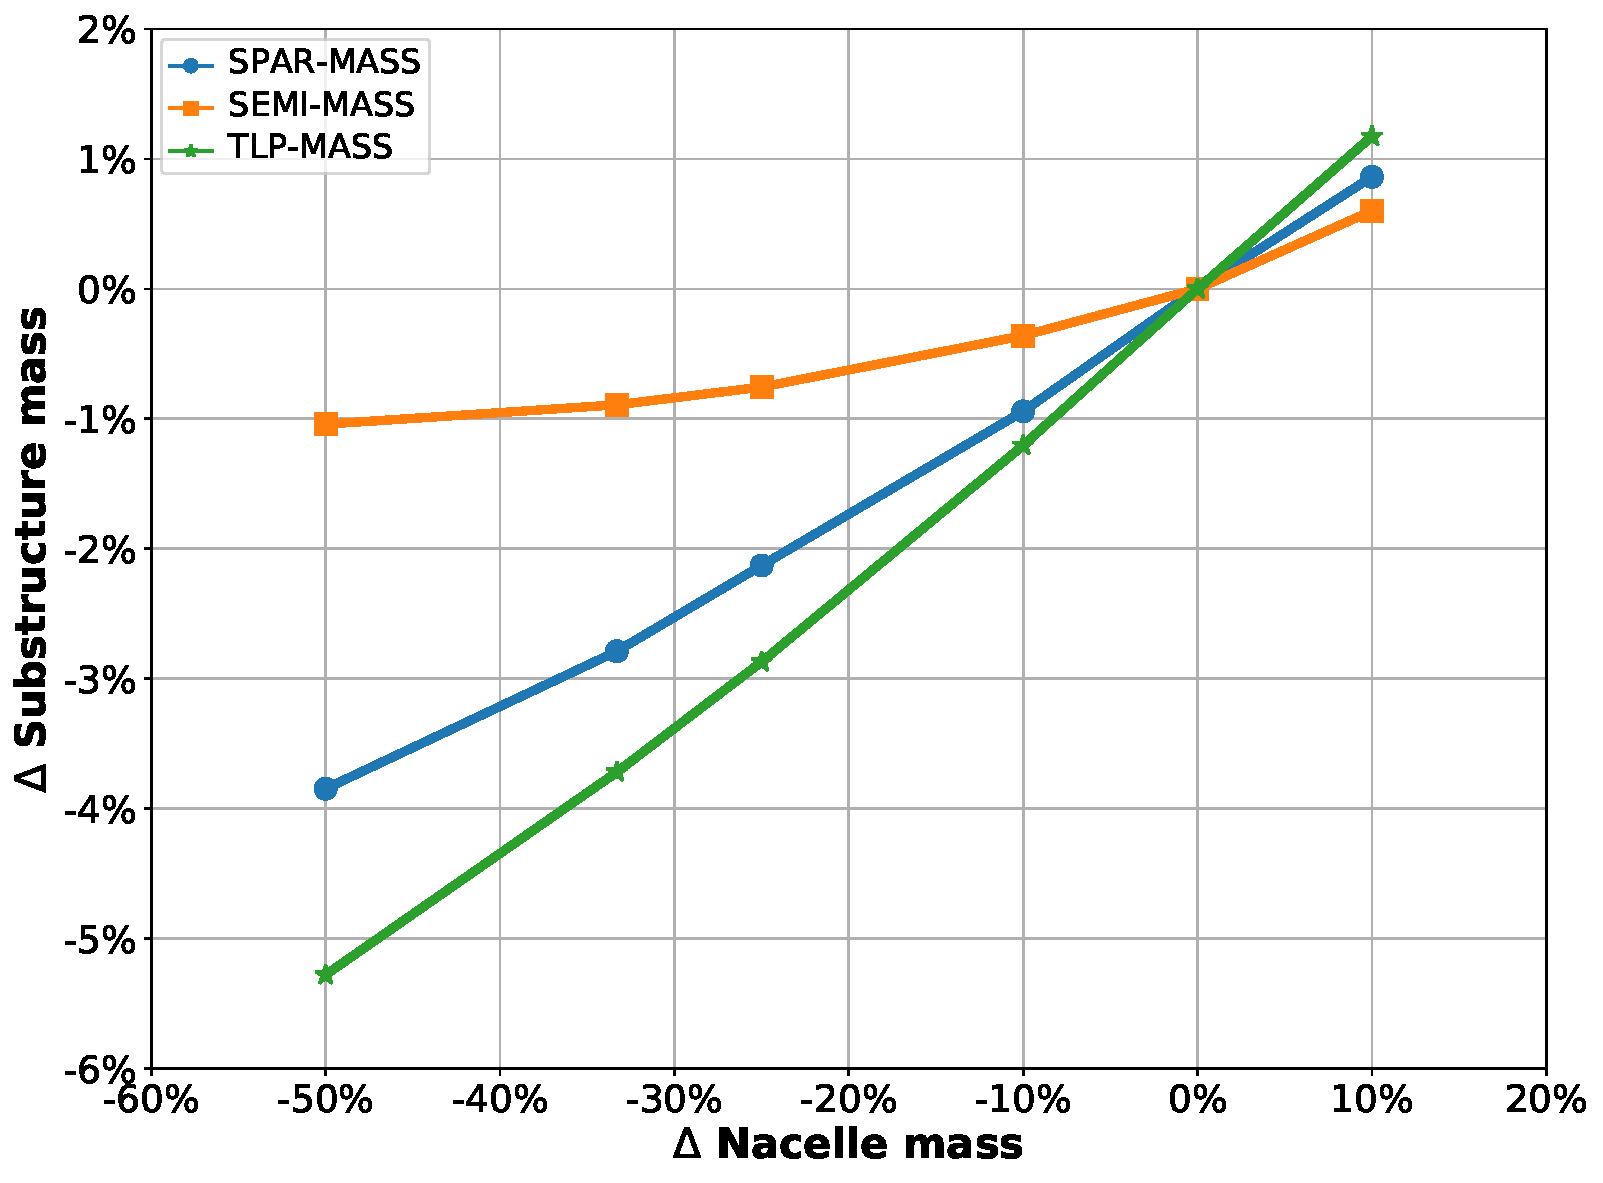
\includegraphics[width=0.9\textwidth]{mass-mass_perc}
    \caption{Percent mass changes, mass-optimized}
  \end{subfigure}
  \caption{Sensitivity of substructure mass (without mooring system)
    relative to mass changes in nacelle for mass-optimized baseline designs.}
  \label{fig:mass-mass}
\end{figure}

The mass sensitivities, shown in
Figure \ref{fig:mass-mass}, are really summary statistics as the
substructure is comprised of multiple components.  The percentage change
of some other metrics are shown in Figure \ref{fig:mass-other}.  Note
that the curves for these other metrics are not smooth because they were
not the objective function, so they were not monitored or controlled by the
algorithm.  For instance, the total displacement (Figure
\ref{fig:mass-other}a), the submerged volume of the substructure, does
not follow the same trend lines as the mass reductions in Figure
\ref{fig:mass-mass}b.  The total displacement of the spar does decrease
as the mass of the nacelle decreases, meaning the tapered column becomes
narrower, but the trend is not nearly as linear as the mass sensitivity.
This is likely due to the fact that the total displacement is closely
tied to some of the stability constraints, such as metacentric height,
and so cannot vary in the same regard.

\begin{figure}[htb]
  \begin{subfigure}[b]{0.49\linewidth}
    \centering 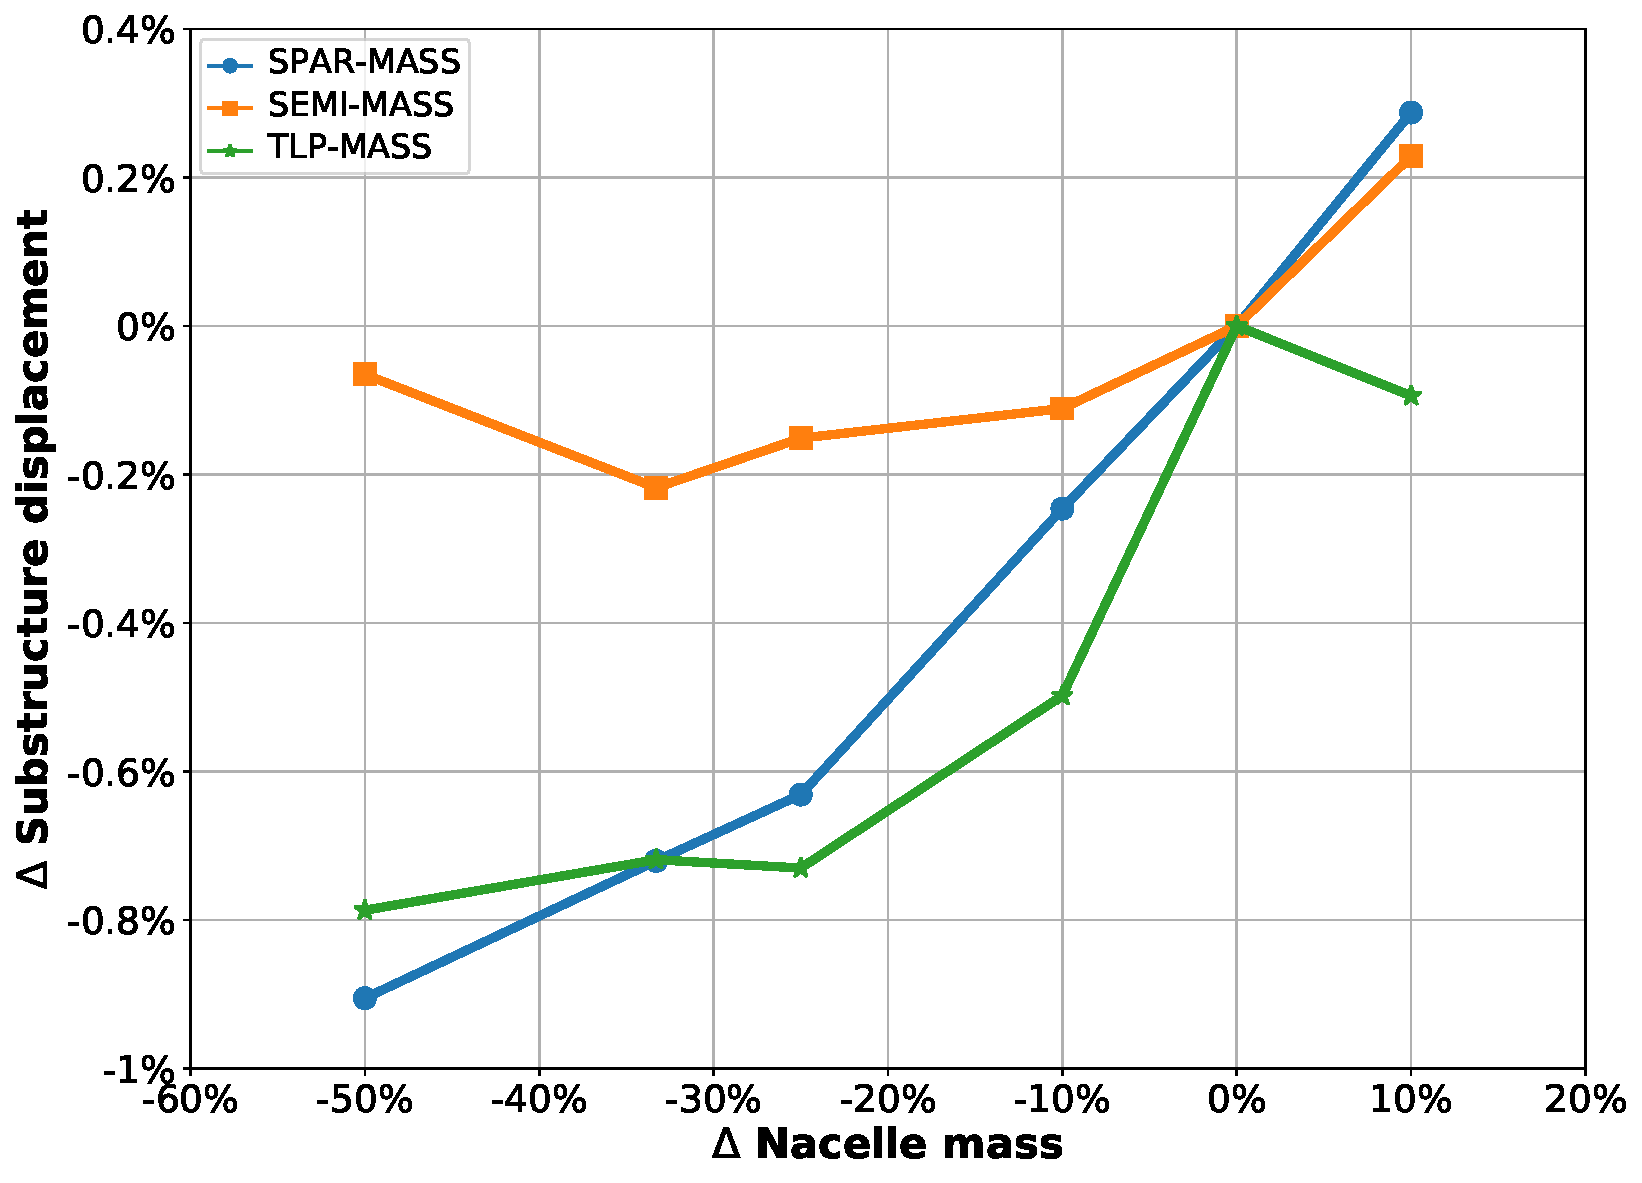
\includegraphics[width=0.9\textwidth]{mass-volume_perc}
    \caption{Displaced volume}
  \end{subfigure}
  \begin{subfigure}[b]{0.49\linewidth}
    \centering 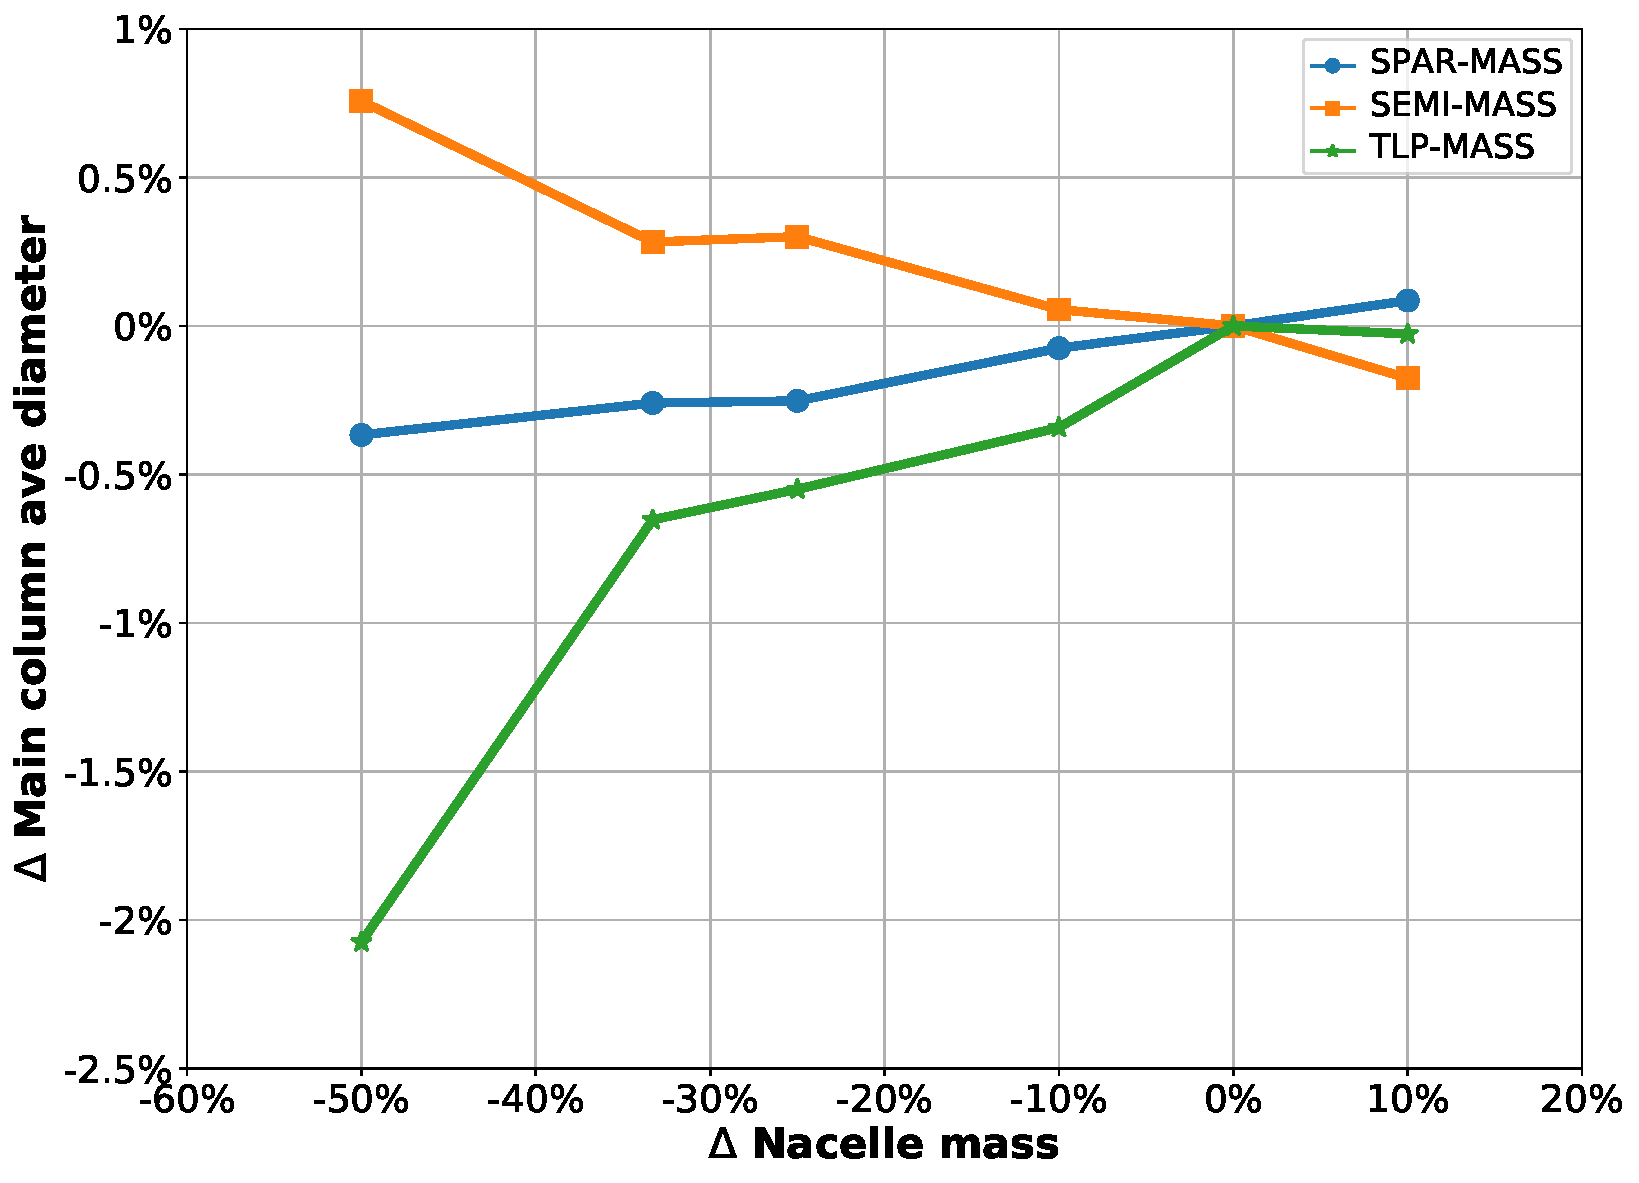
\includegraphics[width=0.9\textwidth]{mass-baseaved_perc}
    \caption{Main column average diameter}
  \end{subfigure}\\
  \begin{subfigure}[b]{0.49\linewidth}
    \centering 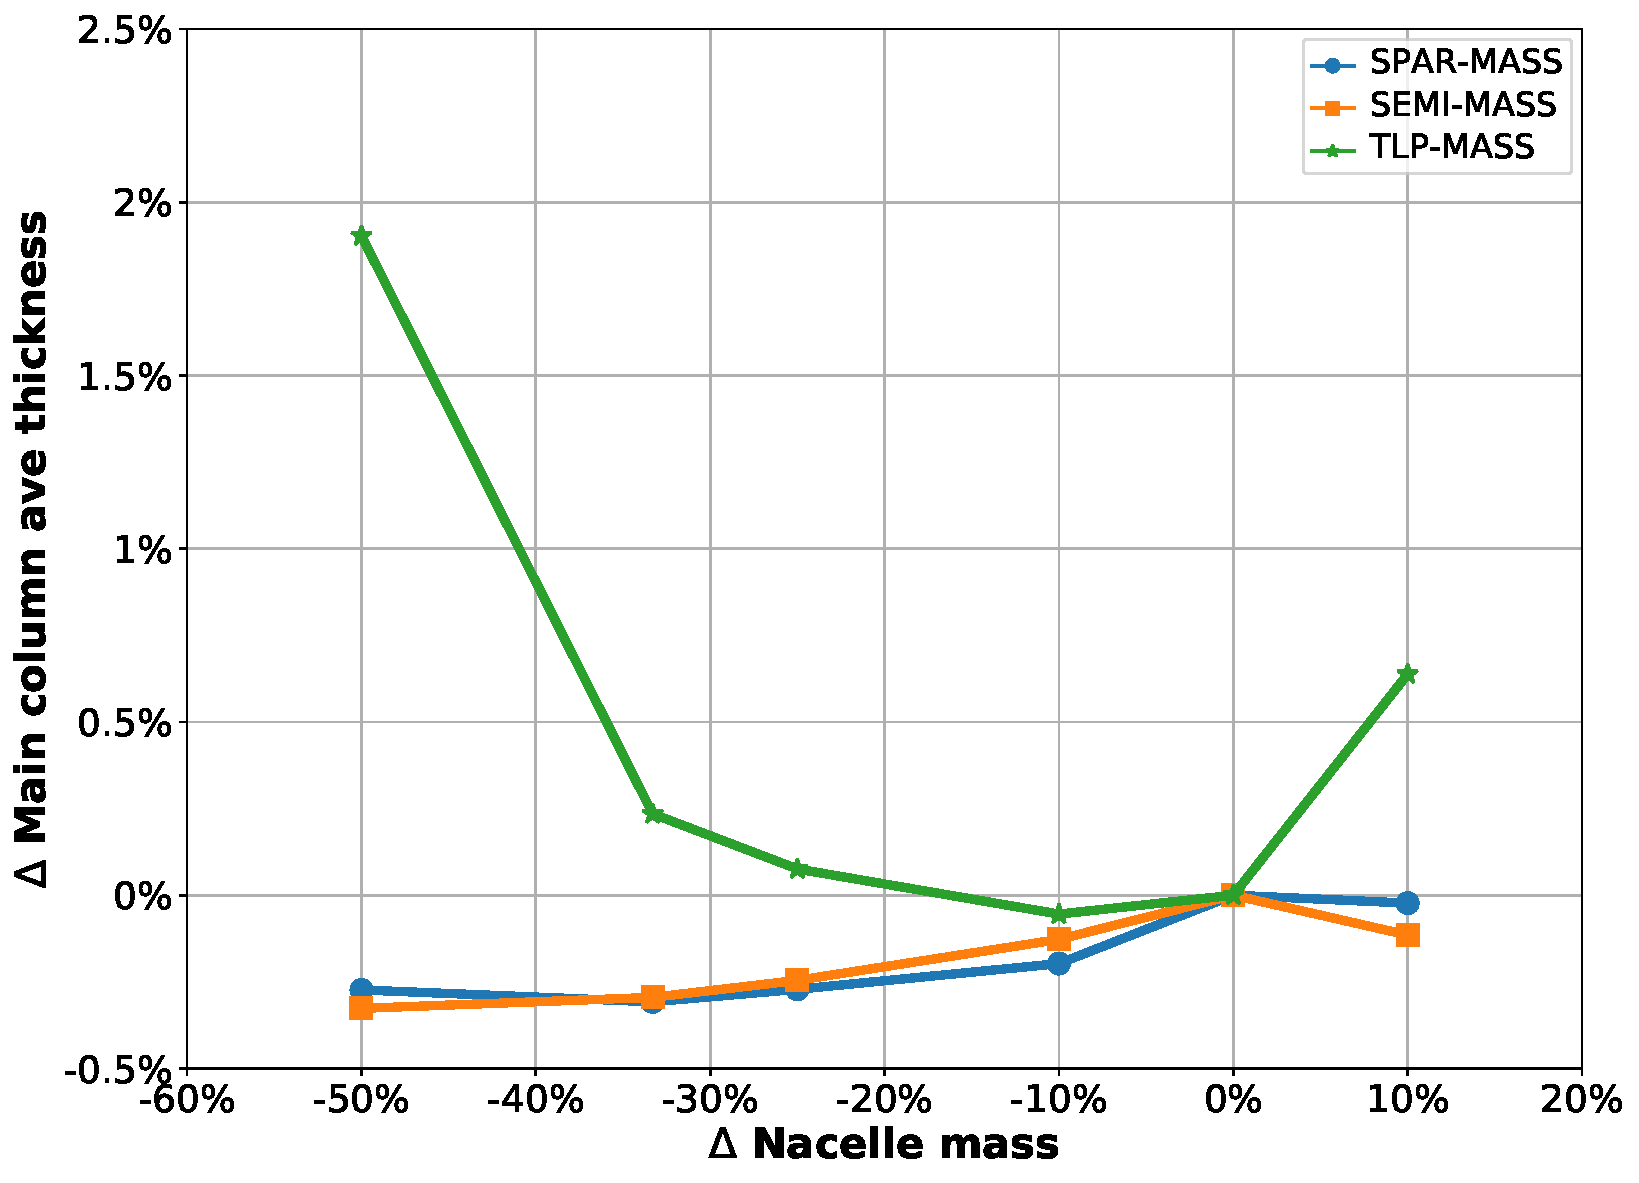
\includegraphics[width=0.9\textwidth]{mass-baseavet_perc}
    \caption{Main column average thickness}
  \end{subfigure}
  \begin{subfigure}[b]{0.49\linewidth}
    \centering 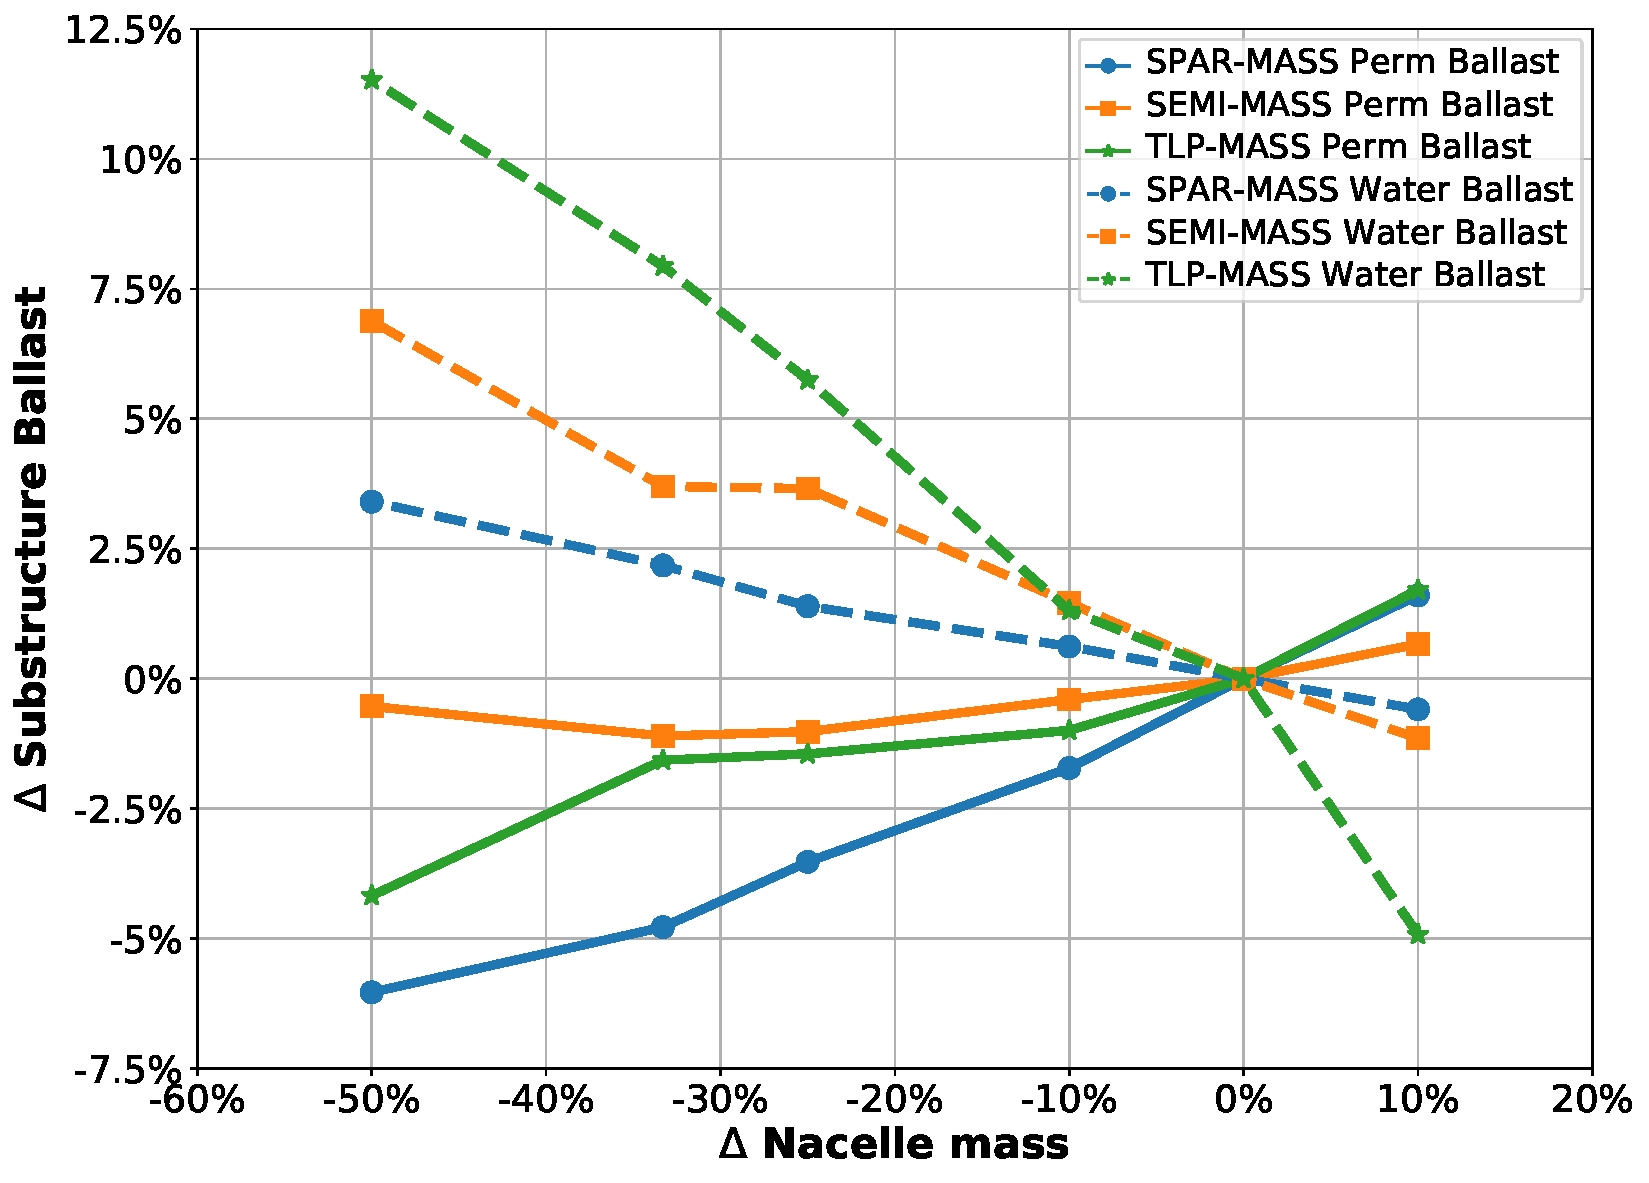
\includegraphics[width=0.9\textwidth]{mass-allball_perc}
    \caption{Permanent (solid) and water (dashed) ballast}
  \end{subfigure}
  \caption{Sensitivity of other substructure metrics (volume, water
    ballast, mooring tension, total cost) relative to mass changes in
    nacelle for mass-optimized baseline designs.}
  \label{fig:mass-other}
\end{figure}

Figures \ref{fig:mass-other}b--c show the change in the average diameter
and thickness of the main column to illustrate how the geometry changes
during the parameterized.  For the spar, as the mass of the nacelle
becomes less, the column becomes both slightly narrower and with
slightly thinner walls.  For the semisubmersible, the diameter stays
roughly constant (or even increases slightly), but the thickness
decreases.  For the TLP, the diameter decreases sharply, but the
thickness increases.

Figure \ref{fig:mass-other}d shows the change in permanent (solid lines)
and water (dashed lines) ballast as the mass in the nacelle decreases.
The percentage changes here are the most pronounced and the shape of the
curves most closely resemble that of the overall mass change in Figure
\ref{fig:mass-mass}b.  This suggests that further converting permanent
ballast into water ballast (which is not counted in the mass budget) is
the dominant trend driving the results of the mass-optimized sensitivity
study.  This is an important trend to keep in mind when interpreting the
change in substructure costs presented below.


\subsubsection{Mass vs.~Cost Scaling}

\begin{figure}[htbp]
  \begin{subfigure}[b]{0.49\linewidth}
    \centering 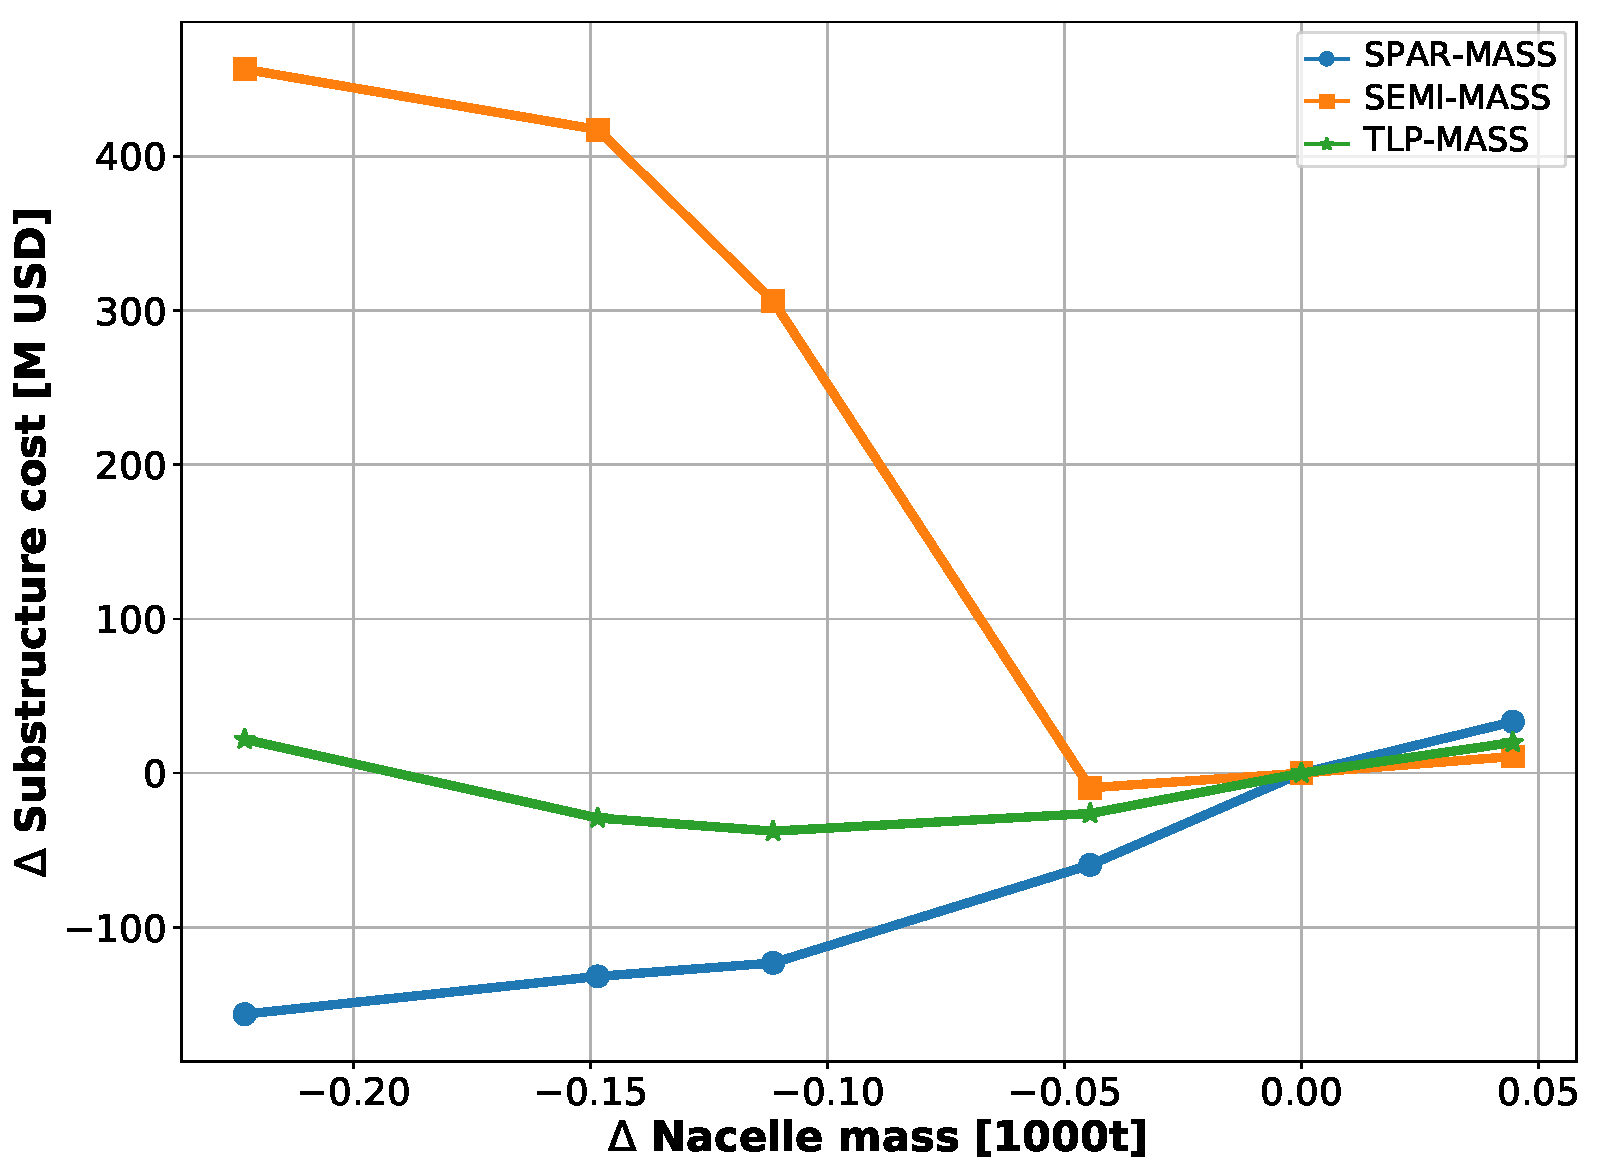
\includegraphics[width=0.9\textwidth]{mass-cost}
    \caption{Absolute cost changes, mass-optimized}
  \end{subfigure}
  \begin{subfigure}[b]{0.49\linewidth}
    \centering 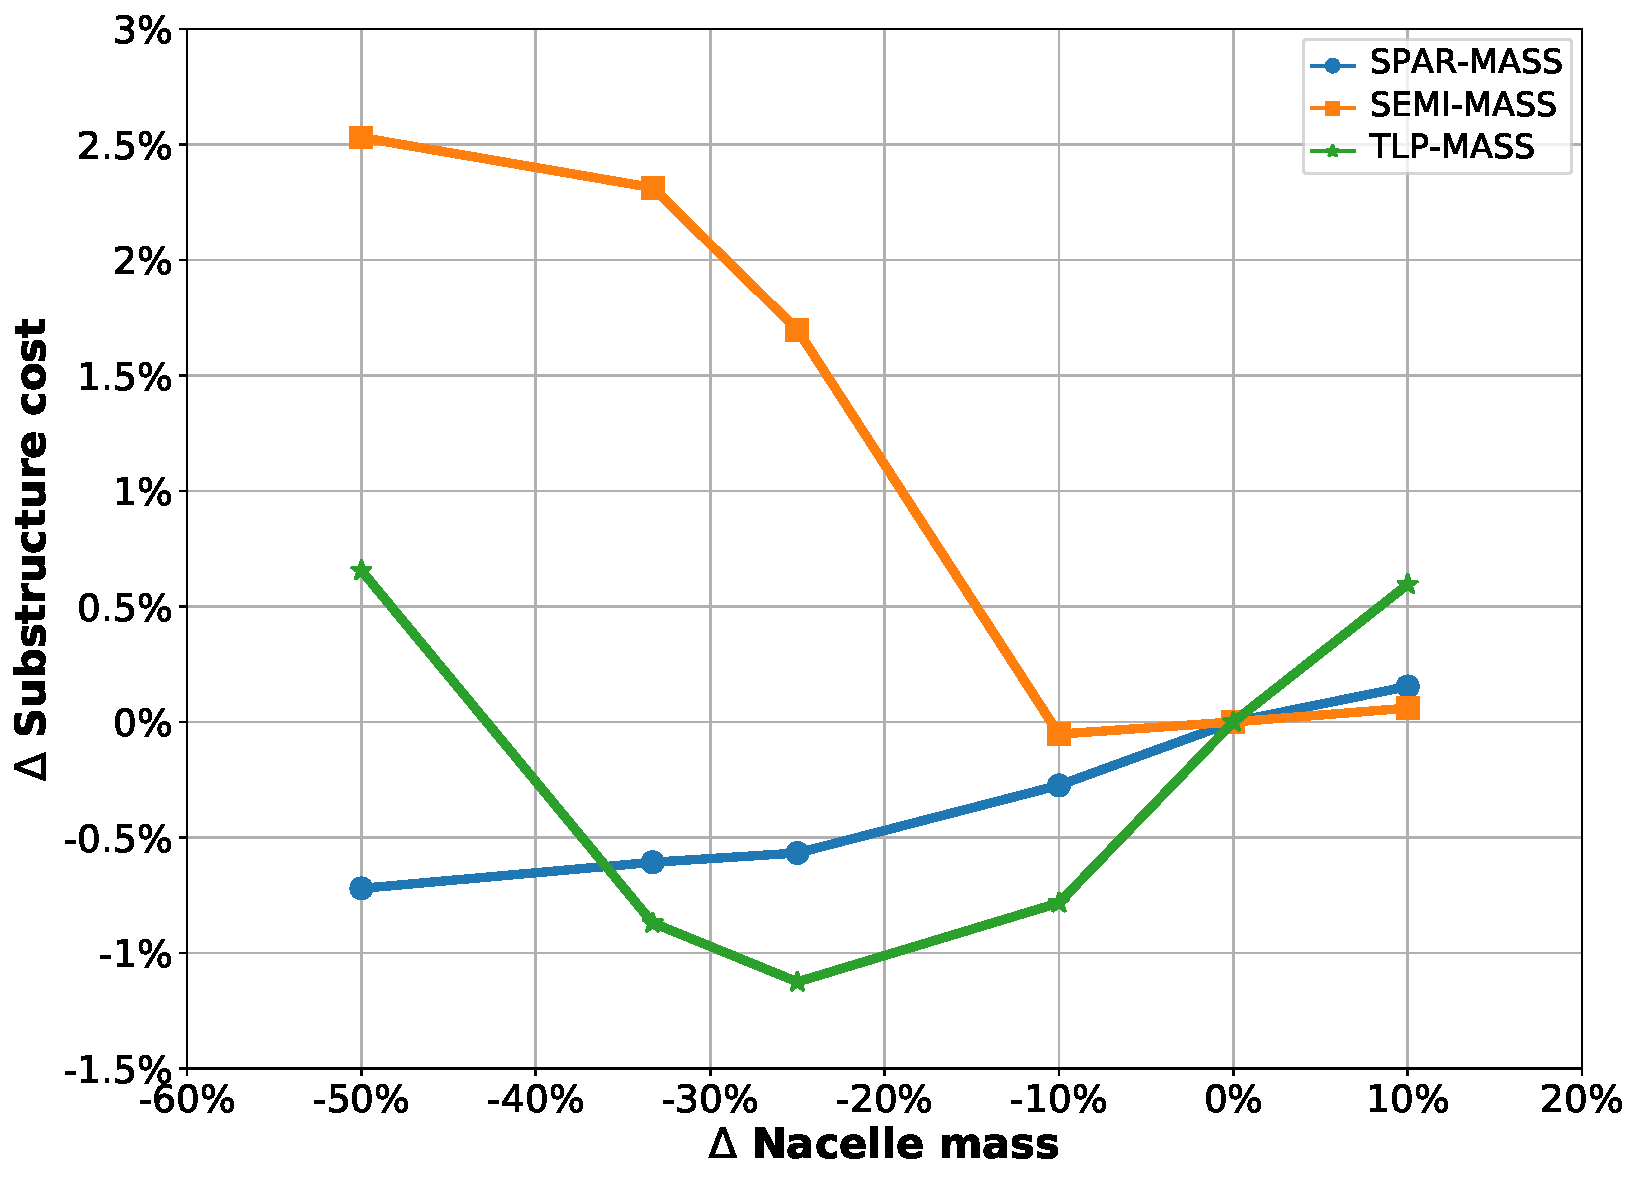
\includegraphics[width=0.9\textwidth]{mass-cost_perc}
    \caption{Percent cost changes, mass-optimized}
  \end{subfigure}\\
  \caption{Sensitivity of substructure cost (with mooring system)
    relative to mass changes in nacelle for mass-optimized baseline designs.}
  \label{fig:mass-cost}
\end{figure}

The change in substructure cost, including the mooring system, for the
mass-optimized designs in the sensitivity study is shown in Figure
\ref{fig:mass-cost} in both absolute and percentage terms.  The results
are, at first, quite surprising, but are consistent with the other
results shown above.  The mass-optimized spar design demonstrates a
mass reduction slope of $1.5--2$ relative to nacelle mass reduction,
which is a reflection of decreases in the spar diameter, thickness, and
permanent ballast.  This leads to a net cost savings of approximately
\$150M for a 50\% reduction in nacelle mass, which is less than 1\% of
the total cost and far from the 4\% reduction in substructure mass.  The
mass-optimized TLP design shows negligible cost savings for all nacelle
mass perturbations, despite a consistent mass reduction slope of $1$.
The mass-optimized semisubmersible design has a small margin for overall
mass reduction since it is tightly constrained, but nevertheless does
achieve measurable reductions over the course of the parameterization.
However, Figure \ref{fig:mass-cost} shows that this mass reduction
actually incurs a cost increase.  This is inconsistent with
expectations, but can be understood through the results in Figure
\ref{fig:mass-other}d and Table \ref{tbl:factors}.  To reduce the mass,
the optimizer has aggressively reduced the amount of permanent ballast
in favor of water ballast.  To maintain stability despite this change,
the column diameter and draft (which was not shown) actually increased
slightly.  While permanent ballast is heavy, it is also inexpensive per
unit mass, whereas rolled steel columns are an order-of-magnitude more
expensive.  Since the mass-optimized design is blind to cost, the
algorithm traded a heavy but cheap ingredient for a lighter but more
expensive ingredient.  This explains the ostensibly counter-intuitive
trends seen in Figure \ref{fig:mass-cost}.

\subsubsection{Cost-Optimized Design Sensitivity}
For a consistent reduction in both substructure mass and cost with
respect to mass reductions in the nacelle, we must look to the
cost-optimized design sensitivity results.  These results are shown in
Figure \ref{fig:cost-cost}.  The reductions of platform mass, shown in
Figures \ref{fig:cost-cost}a--b, are quite linear despite the fact that
the designs are cost-optimized.  The slopes of the lines are actually
about equal to those in Figure \ref{fig:mass-mass}.  The spar has a
slope of approximately $2$, and the TLP still has a slope of about $1$.
The semisubmersible line, however, has a much steeper slope, $1.5$, than
in the mass-optimized case.  It is important to note that these
cost-optimized designs have a different baseline starting point than the
mass-optimized designs and all changes shown are relative.  Thus, while
the mass reduction slope for the semisubmersible design is steeper in
Figure \ref{fig:cost-cost} than Figure \ref{fig:mass-mass}, the
mass-optimized design still achieves a lower overall mass.

\begin{figure}[htb]
  \begin{subfigure}[b]{0.49\linewidth}
    \centering 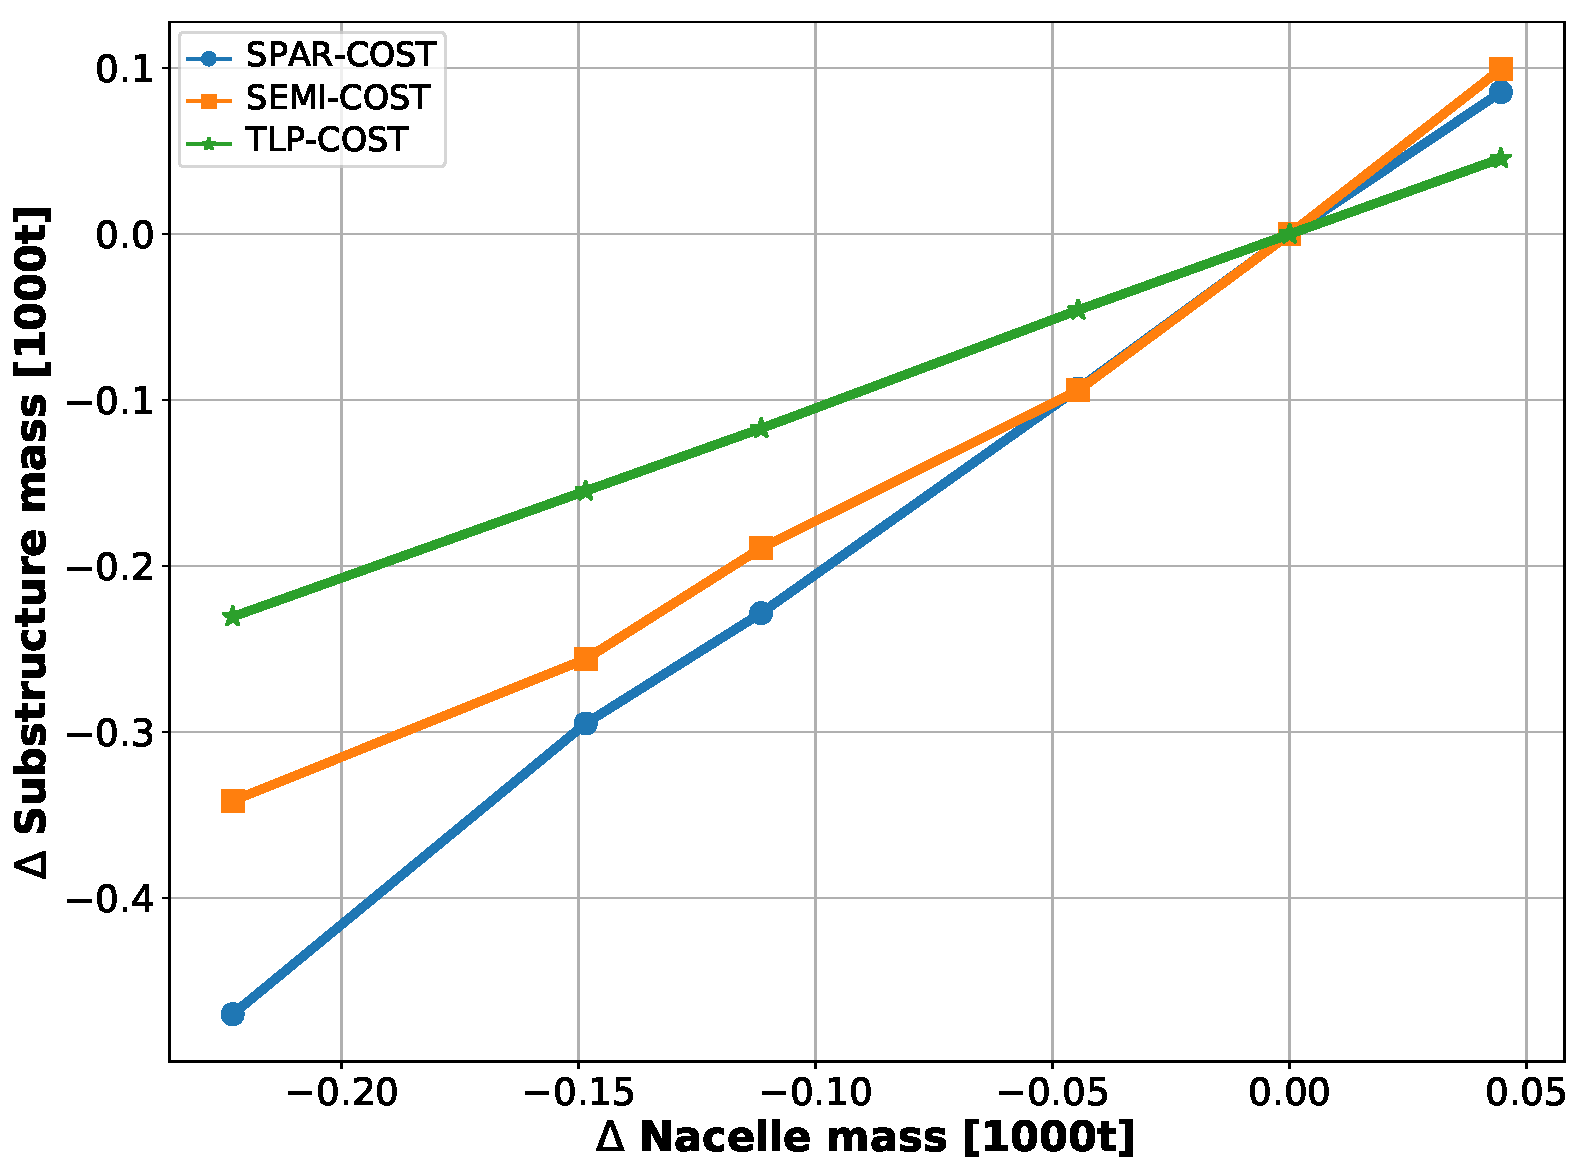
\includegraphics[width=0.9\textwidth]{cost-mass}
    \caption{Absolute mass changes, cost-optimized}
  \end{subfigure}
  \begin{subfigure}[b]{0.49\linewidth}
    \centering 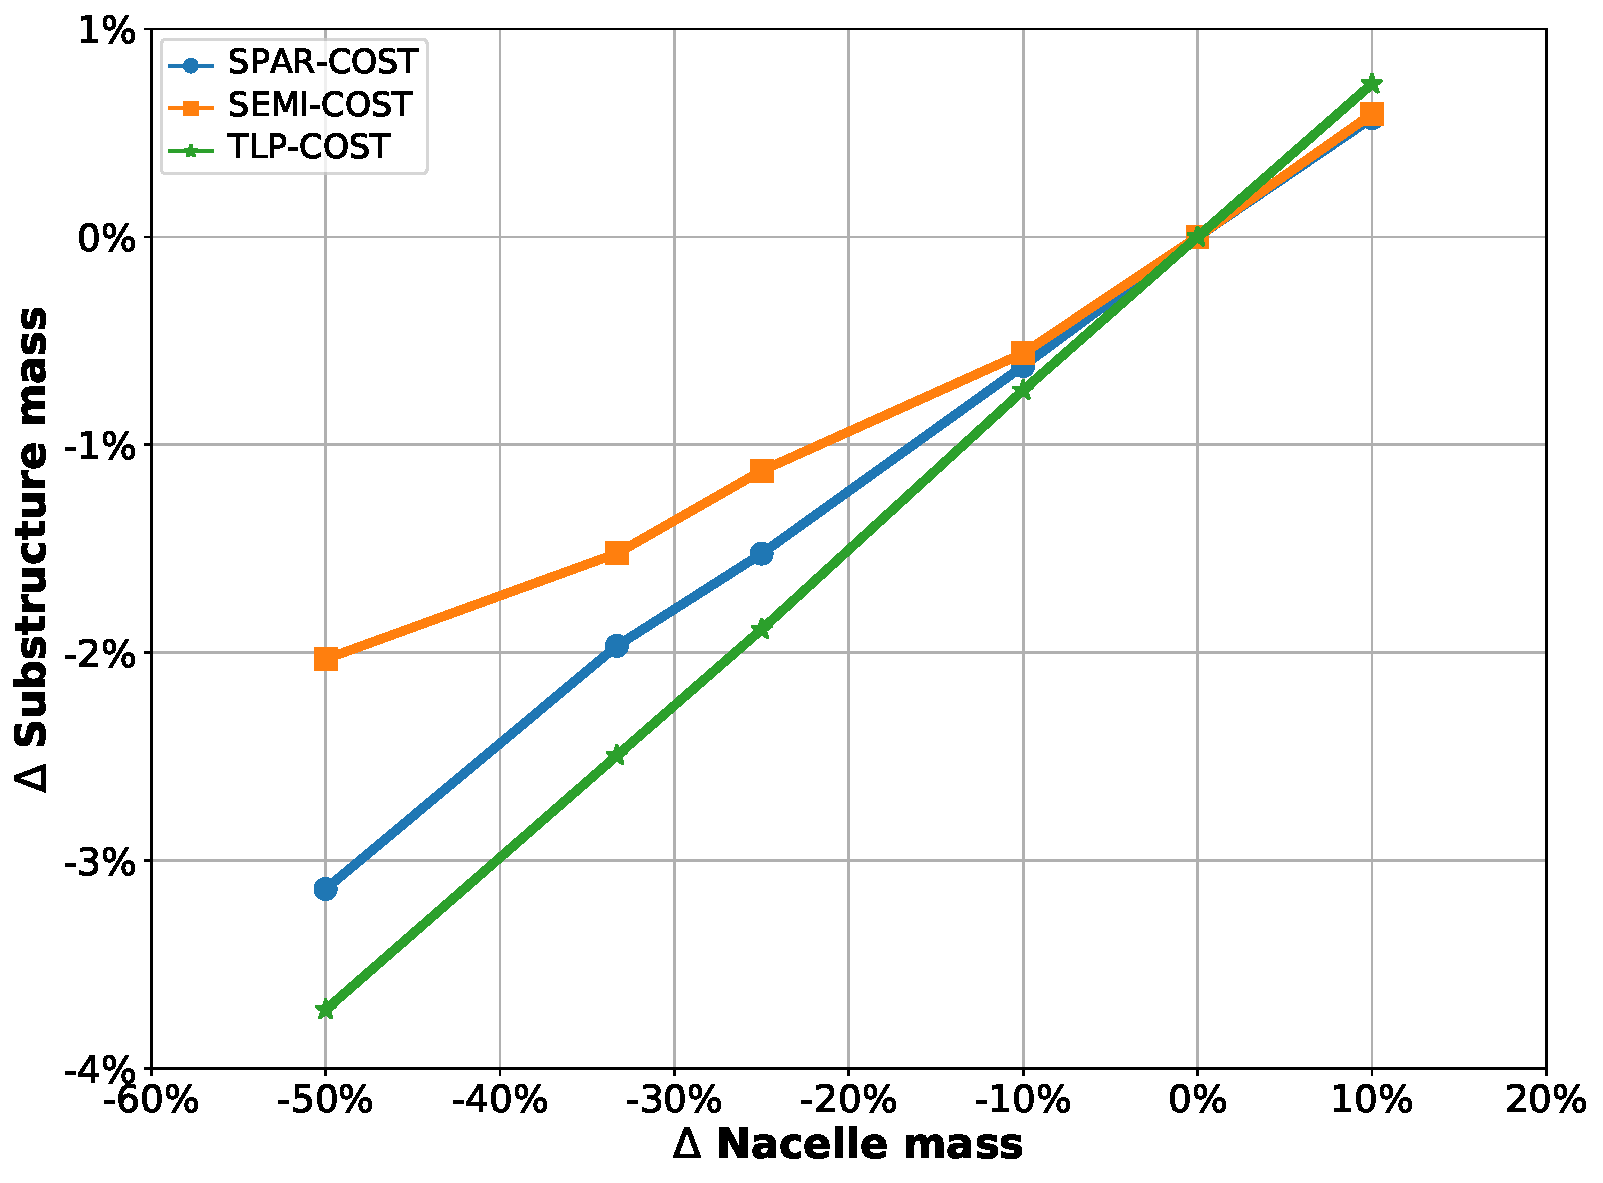
\includegraphics[width=0.9\textwidth]{cost-mass_perc}
    \caption{Percent mass changes, cost-optimized}
  \end{subfigure}\\
  \begin{subfigure}[b]{0.49\linewidth}
    \centering 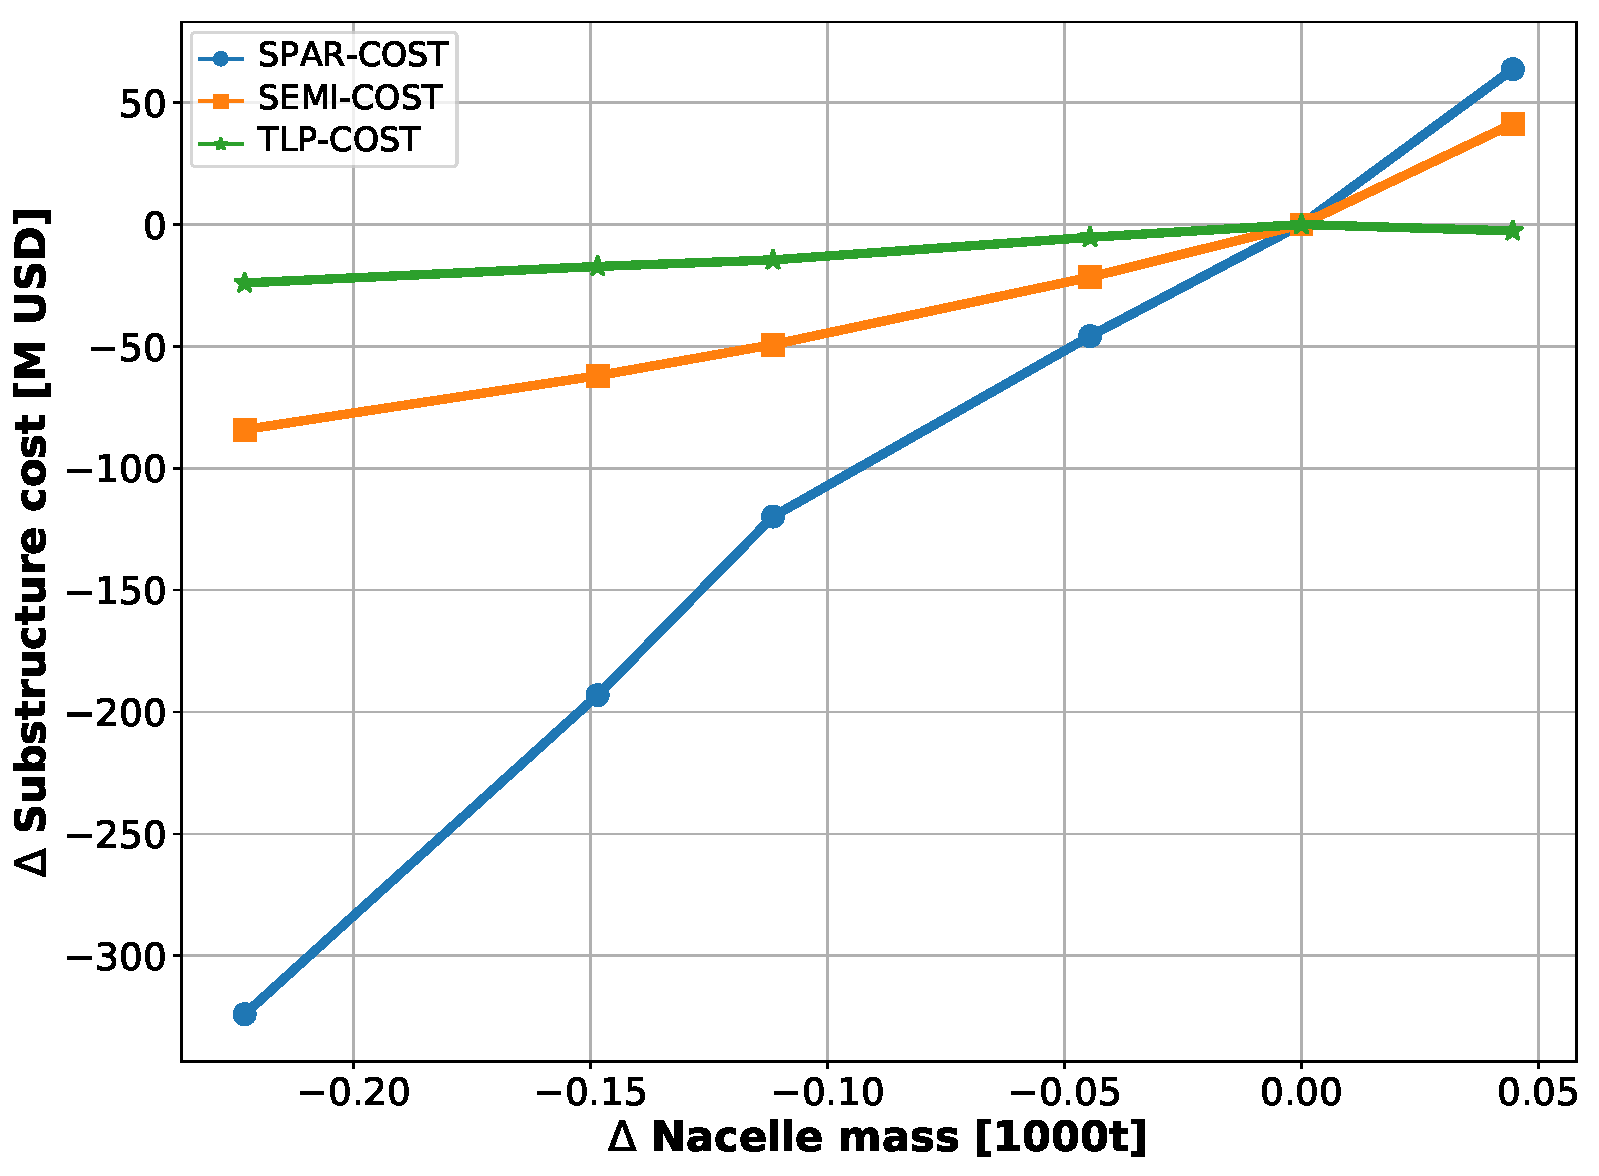
\includegraphics[width=0.9\textwidth]{cost-cost}
    \caption{Absolute cost changes, cost-optimized}
  \end{subfigure}
  \begin{subfigure}[b]{0.49\linewidth}
    \centering 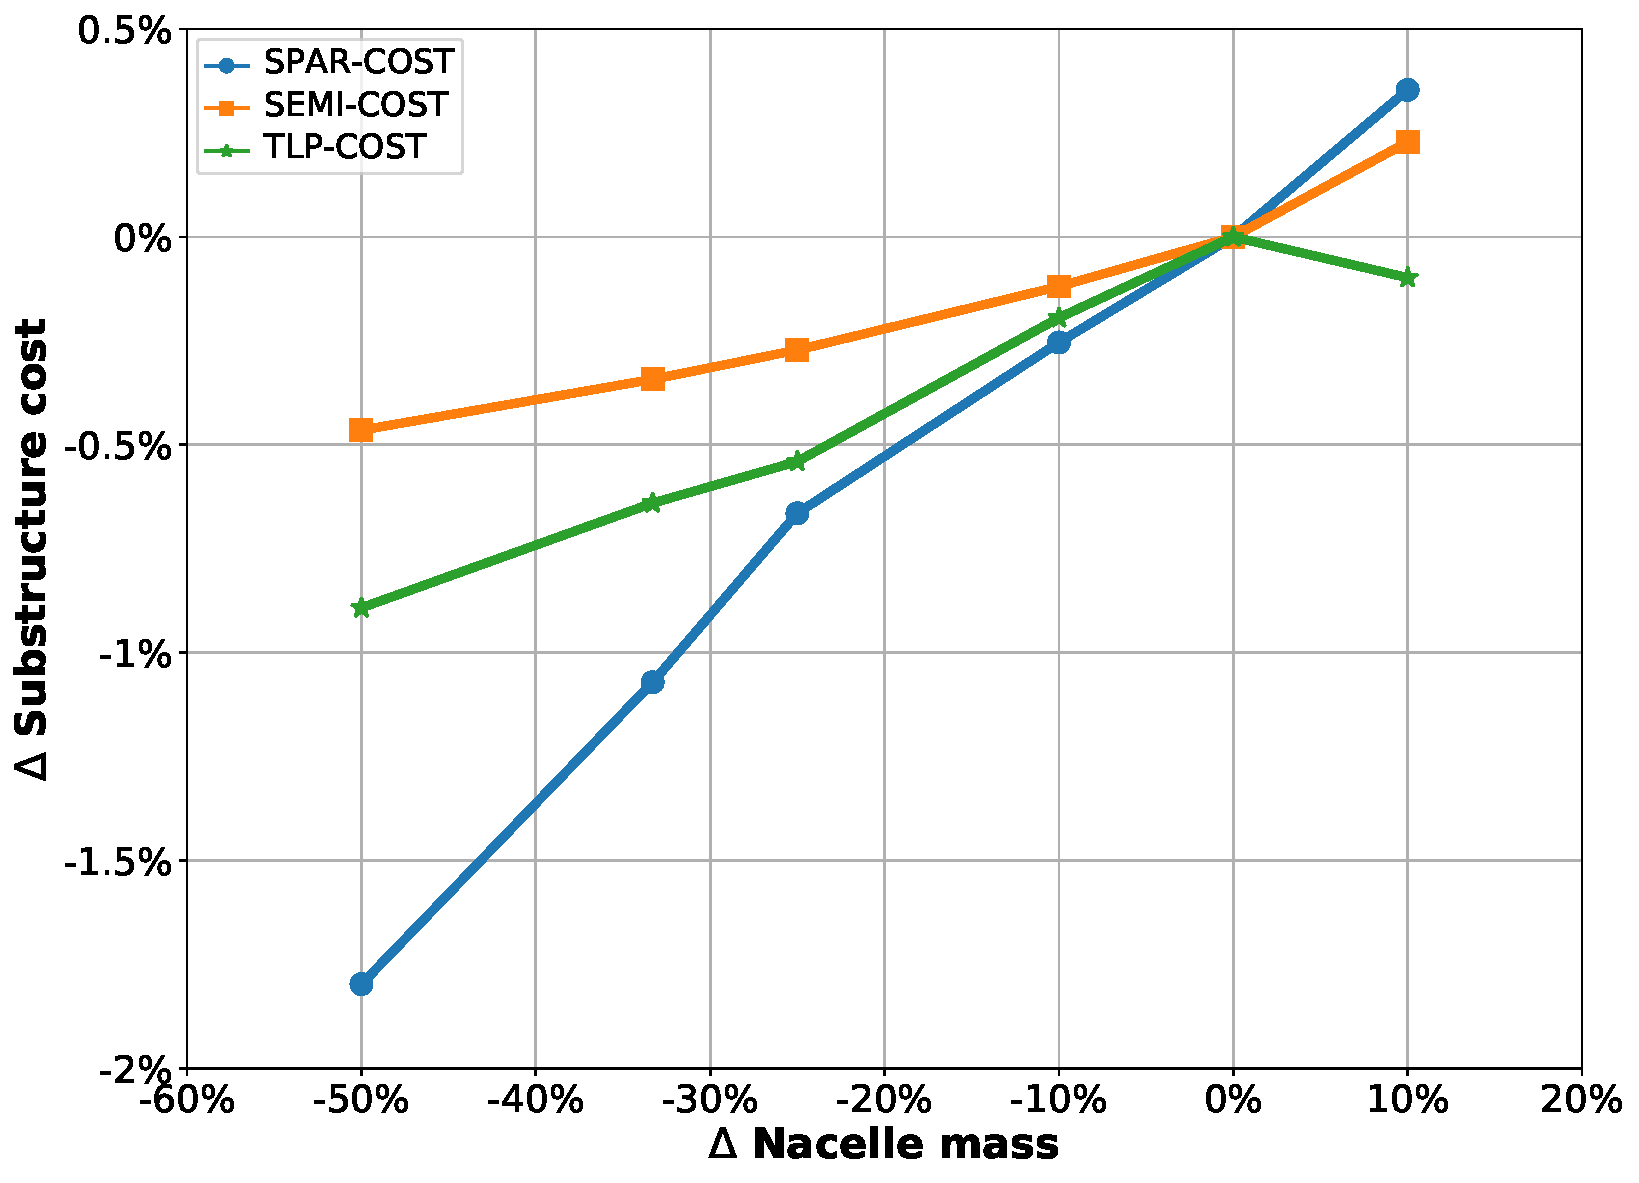
\includegraphics[width=0.9\textwidth]{cost-cost_perc}
    \caption{Percent cost changes, cost-optimized}
  \end{subfigure}
  \caption{Sensitivity of substructure cost (without mooring system)
    relative to mass changes in nacelle for cost-optimized baseline designs.}
  \label{fig:cost-cost}
\end{figure}

The cost reductions for the cost-optimized designs are shown in Figures
\ref{fig:cost-cost}c--d.  Here, at least, there is a consistent cost
decrease, although by percentage it is still far
from the percentage mass decrease.  This is once again explained by the
difference in cost rates among the different components.

The results shown in Figures \ref{fig:mass-cost}-\ref{fig:cost-cost}
have some broader applications than for the immediate study presented
here.  In many engineering studies, mass is used as a surrogate for
capital cost since the development of cost models usually requires a
different set of expertise and input data than what is required for
engineering models.  The implications of the result shown in
Figure \ref{fig:mass-cost} is that mass minimization is not necessarily
a perfect surrogate for capital cost minimization in all cases.  In our
case, the different cost rates for different components means a
mass-focused objective function targets different changes than a
cost-focused objective function.  In other cases, perhaps with
sophisticated cost models that account for various alternative
manufacturing and logistical processes, mass is simply no longer an
adequate surrogate for cost.  Regardless, this observation underscores
some of the messages conveyed in Section \ref{sec:intro} that
advocate for a multidisciplinary systems framework that uses lifecycle
costs to ascertain holistic cost reduction pathways.


\subsection{Break-Even Cost Point for Nacelle Mass Reduction}
One of the more interesting nuggets that can be derived from this type
of design sensitivity study is the cost point required for the
mass-reducing technology (in this case in the drivetrain) to break-even
with the cost changes incurred through the system redesign.  Meaning,
removing mass from the nacelle through the introduction of a new
technology likely comes with a cost premium.  This extra cost, however,
can be offset when the mass savings are propagated through the rest of
the system to reduce structural mass and (hopefully) cost.

\begin{figure}[htbp]
  \begin{center}
    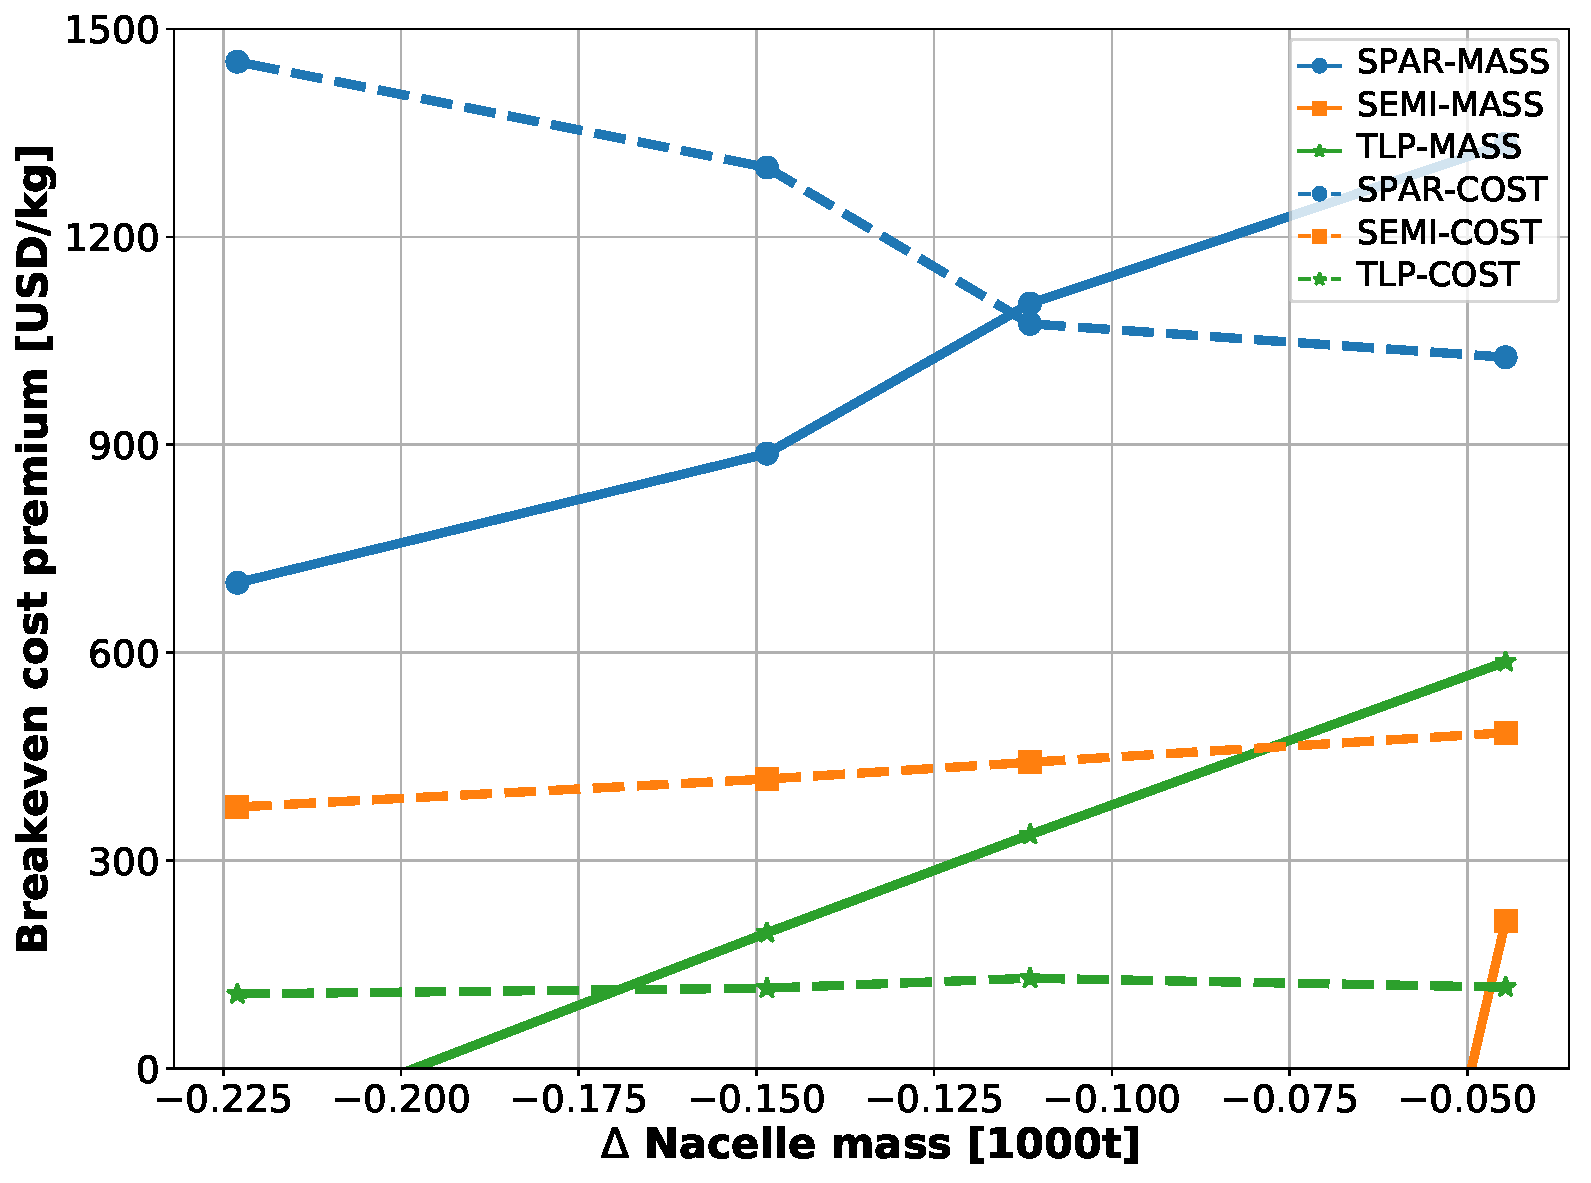
\includegraphics[width=3.5in]{all-premium}
    \caption{Break-even cost premium for the introduction of new drivetrain
      technology.}
    \label{fig:premium}
  \end{center}
\end{figure}

The calculated break-even cost points, for both mass- and cost-optimized
designs, are shown in Figure \ref{fig:premium}.  For the spar designs,
both mass- and cost-optimized, the break-even cost for new drivetrain
technology is approximately \unit[700--1400]{USD/kg}, with a narrower
window for the cost-optimized.  Meaning, if the cost premium to nacelle
mass reduction ratio of the new technology is greater than this value,
then there would be a net cost increase to the system.  If the ratio is
less than this range, then there would be a net cost reduction to the
system.  If the ratio lies within this range, then a little more
detailed investigation would be necessary.

The mass-optimized TLP break-even cost ranges from
\unit[0--600]{USD/kg}, which is a significant variation from
\textit{never worthwhile} to \textit{worthwhile}.  Recall that the cost
reduction in Figure \ref{fig:mass-cost} for the TLP was essentially flat
for reasons already explained.  This is what is driving the inconclusive
determination of the break-even point.  For the same reason, the
mass-optimized semisubmersible design hardly appears in the visual
region of Figure \ref{fig:premium}.

For the cost-optimized semisubmersible and TLP, the break-even results
are much more consistent.  For the semisubmersible, the break-even
cost-ratio is approximately \unit[400--500]{USD/kg} and for the TLP the
value is only about \unit[100]{USD/kg}, a difficult threshold to meet.
Thus, the break-even cost point is dependent on the type of substructure
for this application, hypothetical drivetrain improvement technologies,
and likely other technologies too.

